\documentclass{article}
\usepackage{graphicx}
\usepackage{booktabs}
\usepackage{xcolor}
\usepackage{array}
\usepackage{geometry}
\usepackage{longtable}
\usepackage{float}  % Required for H
\usepackage{titlesec}
\usepackage{hyperref} 
\newcommand{\sectionbreak}{\clearpage}
 
\geometry{a4paper, margin=1in}
 
\title{Creating Space Technical doc}{\centering}
\author{Real Ant Engineer}
\date{May 2026}
 
\begin{document}
 
\maketitle

\newpage
This is a document went to give an overview of the Creating Space to the Engineer Colony team in particular Artists and Devs.
\newpage

\tableofcontents


\section{Presentation, Goals, and Direction}


Creating Space is my first mod. It is an add-on for Create, inspired by Galacticraft and motivated by two major frustrations I encountered while playing that mod. First, the only planet that could host a space station was the Overworld. Second, the rockets were not customizable; they would have been much more interesting as multiblock ships. As such Creating Space aims to achieve the following goals:

\begin{itemize}
    \item Preserve everything that made Galacticraft great:
    \begin{itemize}
        \item Technological progression through new materials discovered on planets and blueprints found in dungeons.
        \item In-situ resource exploitation using automatic rockets.
        \item Base pressurization.
        \item Space stations.
        \item A balance of scientific realism and imaginative fantasy.
    \end{itemize}

    \item Improve and expand on what Galacticraft lacked:
    \begin{itemize}
        \item A coherent lore.
        \item Multiblock-based and fully customizable rockets.
        \item More planets to explore.
        \item More varied landscapes and world generation.
        \item Educational elements that introduce players to celestial mechanics and rocket engineering while remaining accessible to everyone.
        \item Full automation of all crafting processes, as expected in a Create add-on.
    \end{itemize}
\end{itemize}

\section{Rocket}

\subsection{Technical Overview of the Rocket}

The rocket system is designed around a physically inspired propulsion model while remaining practical for gameplay and automation. Rockets are treated as dynamic multiblock vehicles whose performance depends on thrust, mass, fuel consumption, and the selected propulsion system.

Fuel consumption is currently handled through several consumption maps. Each engine defines a mapping between fluid tags and consumption rates derived from the produced thrust. A second scaled consumption map is used during interplanetary travel to ensure that only the amount of propellant corresponding to the required $\Delta v$ is consumed.

The current implementation uses the Tsiolkovsky rocket equation to compute the theoretical $\Delta v$ available to the vehicle:

\[\Delta v = v_e \ln\left(\frac{m_d + m_p}{m_d}\right)\]

where:

\begin{itemize}
    \item $\Delta v$ is the total available velocity change,
    \item $v_e$ is the effective exhaust velocity,
    \item $m_d$ is the dry mass of the rocket (structure, components, and inert fluids),
    \item $m_p$ is the total propellant mass.
\end{itemize}

This equation allows the game to estimate whether a rocket can reach orbit, transfer between planets, or land safely. The consumption map dedoubled, one is used to compute ISP and the othere one is scaled to consume only the amount of propellant required for the computed maneuver.

\subsection{Rocket Menu}

The rocket menu will act as the main interface for configuring and analyzing spacecraft.

One section of the interface is dedicated to rocket analysis. It could displays information such as:

\begin{itemize}
    \item Total mass,
    \item Available $\Delta v$,
    \item Thrust-to-weight ratio,
    \item Fuel reserves,
    \item Estimated reentry heating and thermal limits (Real Ant Engineer has a version i python for reentry simulation)
\end{itemize}

Another section handles destination selection and flight planning. Two navigation modes are planned:

\begin{itemize}
    \item A simple manual destination selector for direct player-controlled launches, could reuse the older destination menu until something better is made.
    \item A scheduling system for automated logistics and cargo transfers, right now used for everythig.
\end{itemize}

The current menu has a bunch of issues including but not limited to a hugly/buggy menu layout. To solve the buggy menu layout we could use the new compound widget created in our formicAPI

\subsection{Maneuvering and Docking}

Orbital maneuvering and station docking are planned for space stations and spacecraft.

Docking operations will likely rely on beacon systems that allow stations to broadcast positional data. Rockets equipped with the appropriate systems could then align automatically or assist the player during docking maneuvers.

Future mechanics may include:

\begin{itemize}
    \item Relative velocity matching,
    \item Assisted docking alignment,
    \item Staging and docking between rockets/ships.
    \item Animation on interplanetary movements
\end{itemize}

\subsubsection{HUD}

A dedicated HUD is planned for spacecraft control and orbital flight.

The interface would display:

\begin{itemize}
    \item Current movement mode,
    \item Rocket orientation,
    \item Linear and relative velocity,
    \item Remaining fuel,
    \item Direction and distance to navigation beacons or stations.
\end{itemize}

\section{Rocket Engine Recipe}

As stated in the introduction, rocket engines should be customizable both to satisfy players who enjoy optimizing their designs and to support a meaningful progression system. At the same time, the system must remain accessible to new players and to those who are less interested in the engineering aspects. In its current state, the mod does not fully achieve either of these objectives.

\subsection{Rocket Engine Components}

\subsubsection{Overview}

\begin{figure}[H]
    \centering
    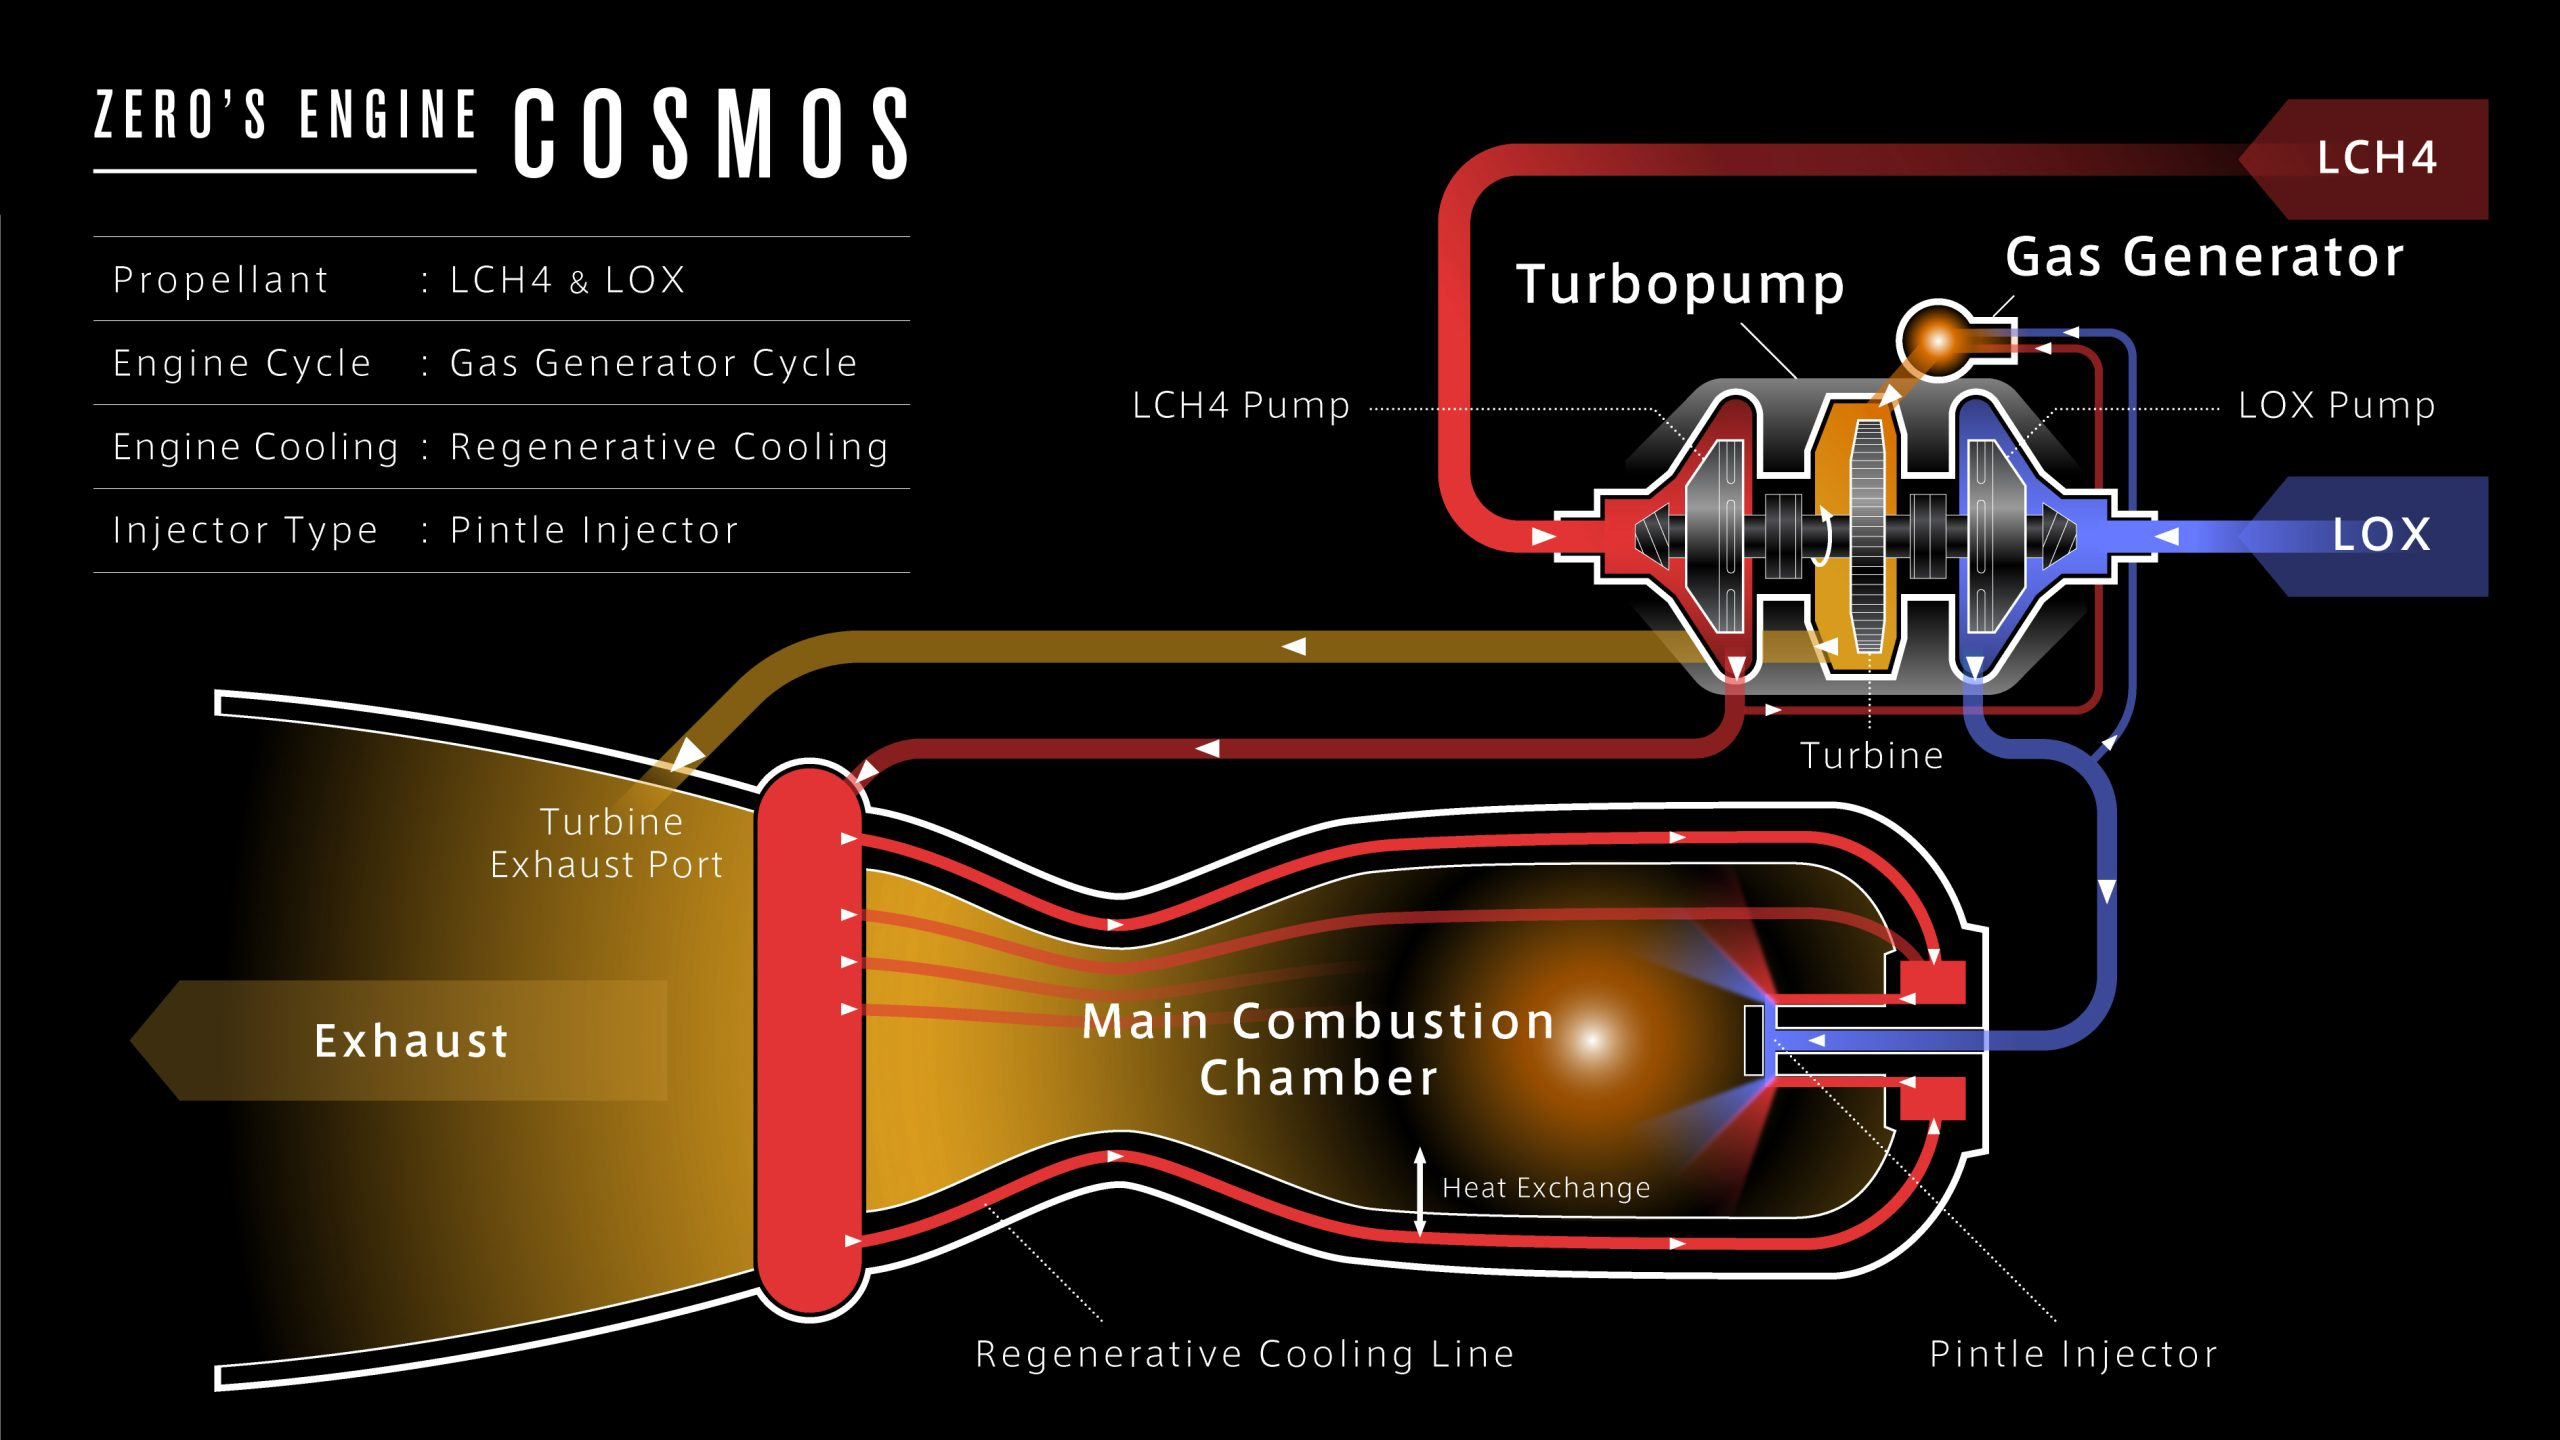
\includegraphics[width=\linewidth]{images/open_cycle_1.png}
    \caption{Overview of an open-cycle rocket engine}
    \label{fig:open-cycle-overview}
\end{figure}

To better understand how the different parts of a rocket engine fit together, Figure~\ref{fig:open-cycle-overview} provides an overview of the main components and their interactions. In an open-cycle engine, a small portion of the propellants is burned in a separate gas generator to power the turbopumps, while the remaining propellants are fed into the main combustion chamber where thrust is produced.

\subsubsection{Turbopump}

\begin{figure}[H]
    \centering
    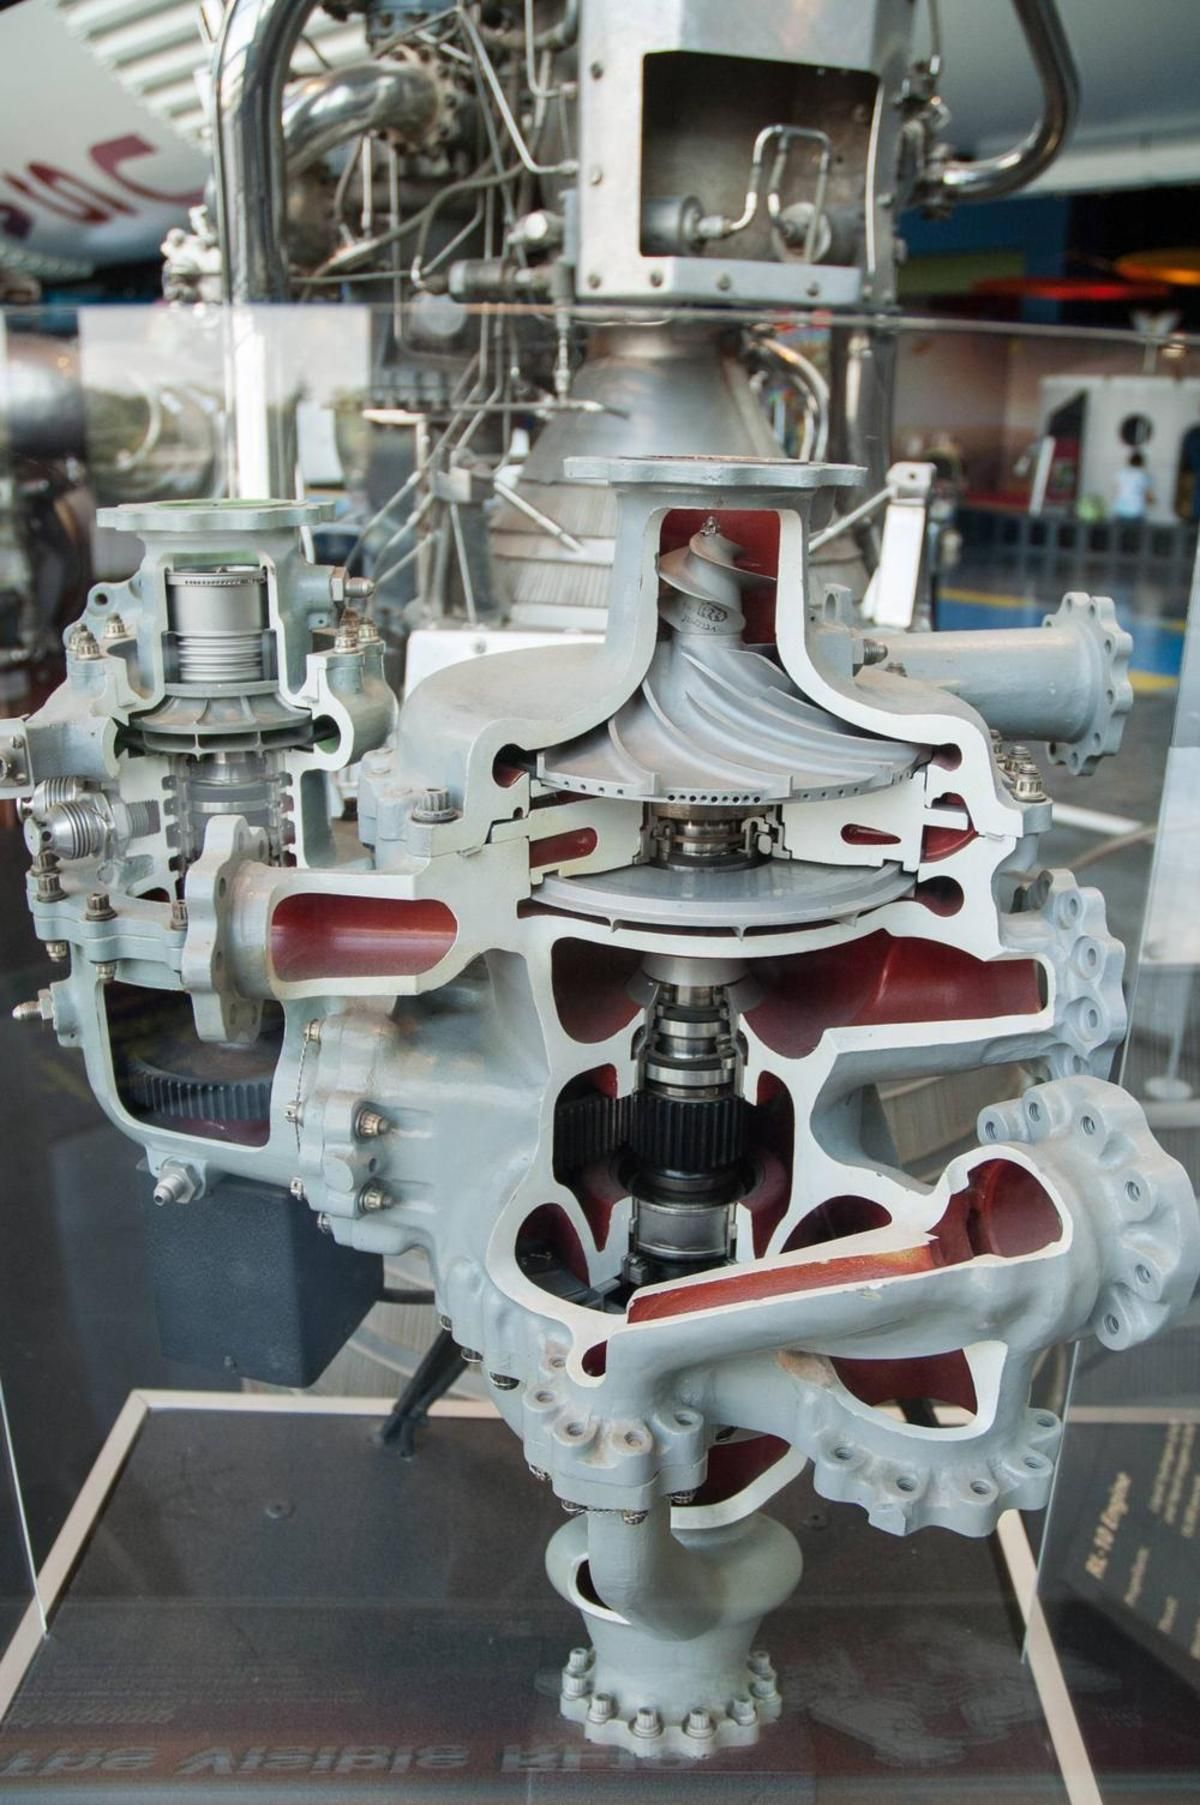
\includegraphics[width=0.75\linewidth]{images/turbopump-slice.png}
    \caption{Twin turbopump with a single turbine}
    \label{fig:turbopump}
\end{figure}

The turbopump is one of the most complex and expensive components of a rocket engine. It is an extremely powerful pump, often delivering tens of thousands of horsepower, driven by a small turbine powered by hot gases. Its role is to feed large quantities of propellant into the combustion chamber at very high pressure.

The design shown in Figure~\ref{fig:turbopump} uses a single turbine to drive two separate pumps: the large pump in the center and a smaller one on the left. The two are connected through a gear train. Although this configuration is mechanically interesting, it is too complex to be implemented directly in the mod in its current state.

\begin{figure}[H]
    \centering
    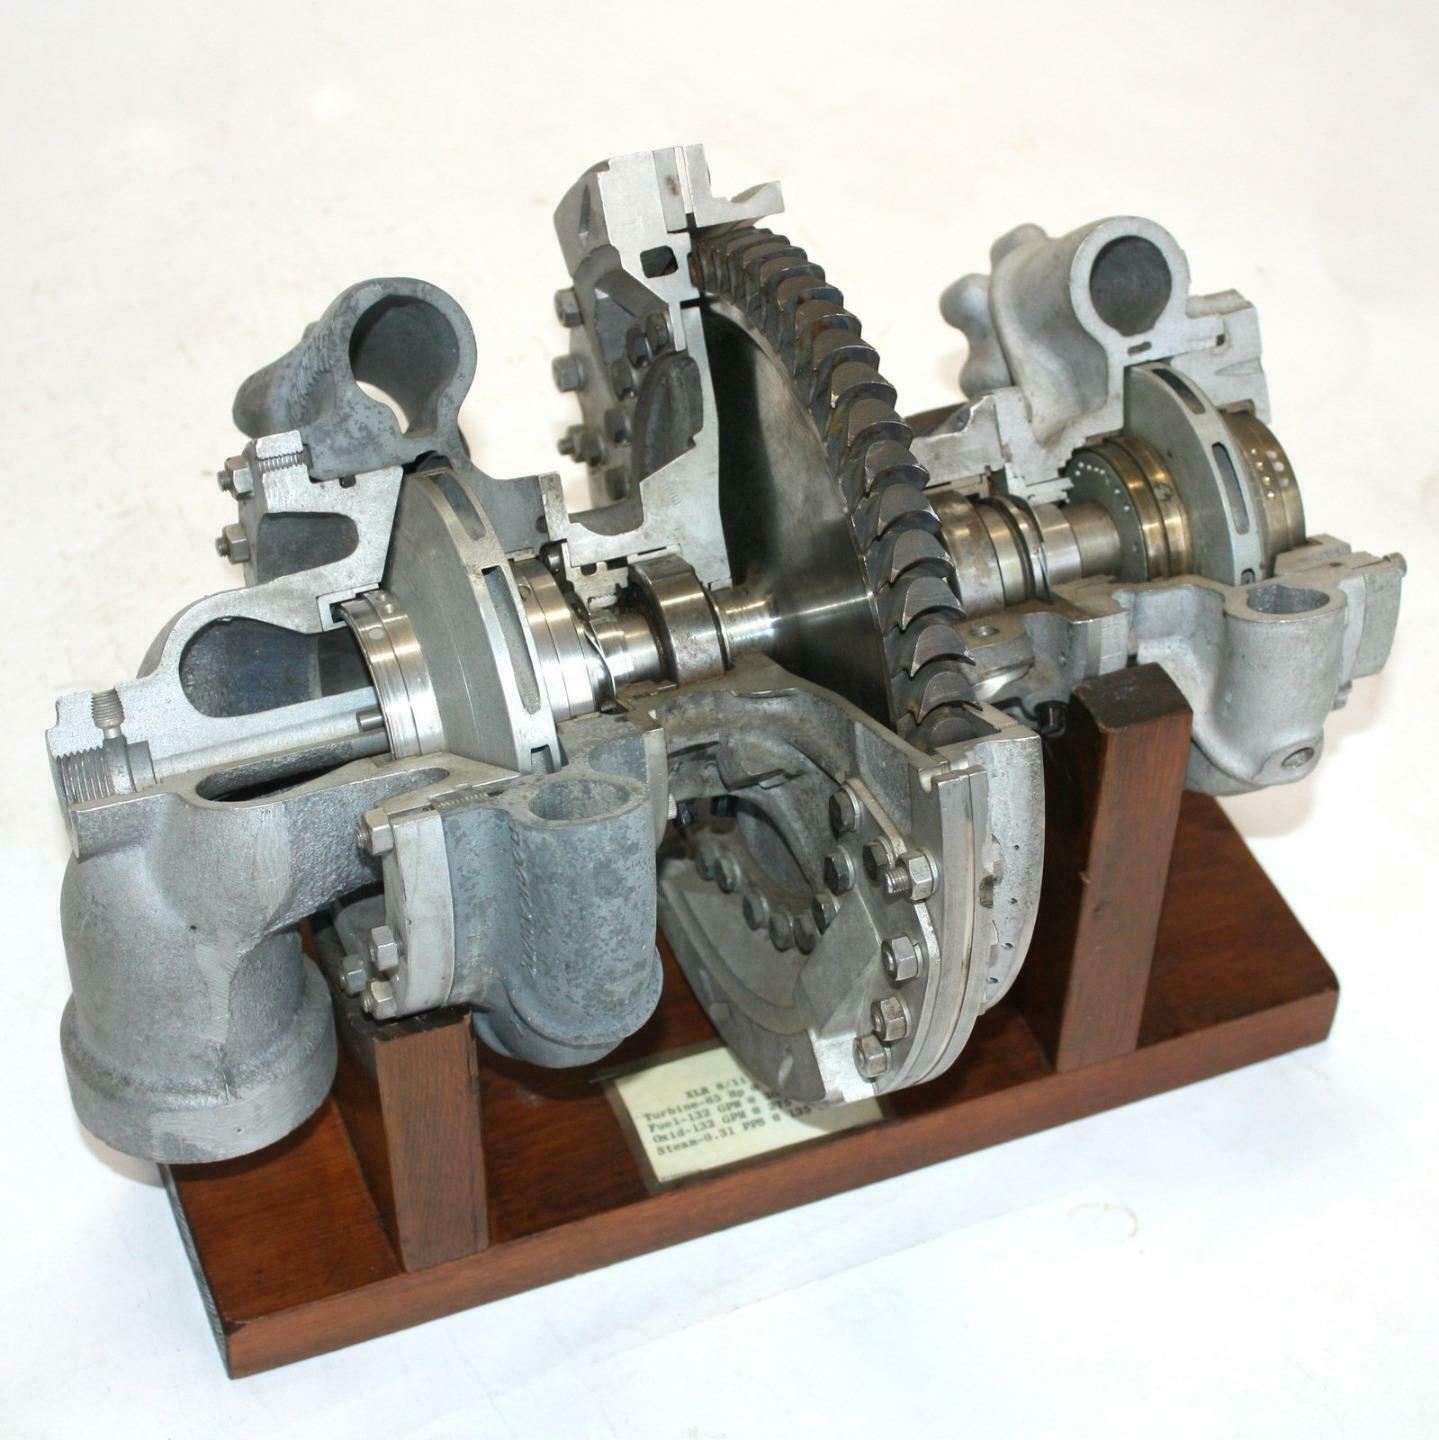
\includegraphics[width=0.75\linewidth]{images/turbopump-slice-2.png}
    \caption{More conventional twin turbopump design}
    \label{fig:turbopump-2}
\end{figure}

A more common arrangement is shown in Figure~\ref{fig:turbopump-2}, where the two pumps are mounted on the same shaft with the turbine located between them. This design is simpler and more representative of what is shown in the GUI.

For additional details on the internal workings of turbopumps, see \href{https://en.wikipedia.org/wiki/Turbopump}{Wikipedia's article on turbopumps}.

\subsubsection{Blisk}



\subsubsection{Injector}

There are almost as many injector designs as there are rocket engineers. The injector selected for the mod is the pintle injector, which is both simple and highly effective.

\begin{figure}[H]
    \centering
    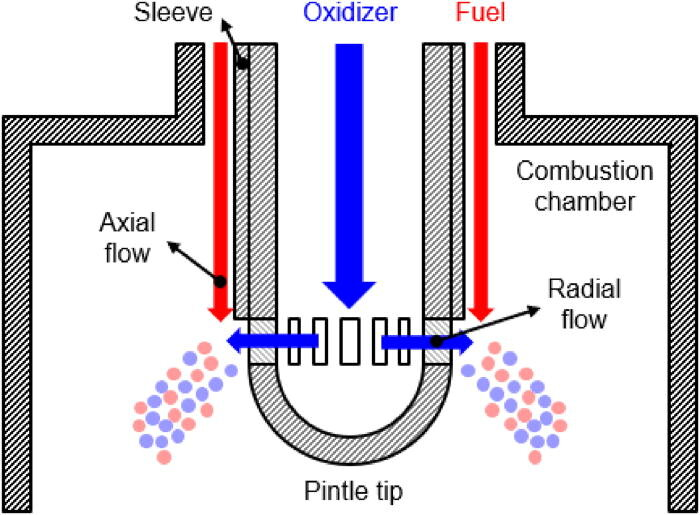
\includegraphics[width=0.50\linewidth]{images/pintle-injector.png}
    \caption{Pintle injector}
    \label{fig:pintle-injector}
\end{figure}

A pintle injector works by injecting one propellant through a central rod while the other flows around it. The two streams collide and mix efficiently, producing stable combustion. This design is particularly attractive because it offers good performance while remaining mechanically straightforward.

\subsubsection{Injector Grid}

\subsubsection{Nozzle}

The nozzle is responsible for converting the thermal energy of the combustion gases into directed velocity, thereby generating thrust.
%% put the expansion ratio explanation here with the isentropic forumals

There are two main nozzle types considered for the mod: the bell nozzle and the aerospike nozzle. Both perform the same fundamental function, but they differ significantly in behavior and engineering challenges.

\begin{figure}[H]
    \centering
    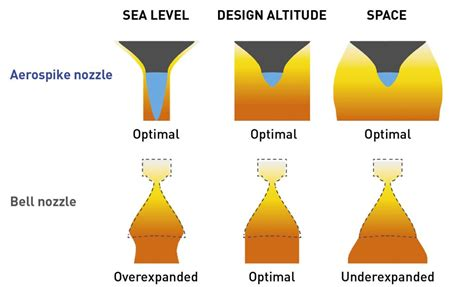
\includegraphics[width=0.75\linewidth]{images/aerospike-vs-bell-nozzle.png}
    \caption{Comparison between aerospike and bell nozzles}
    \label{fig:aero-vs-bell}
\end{figure}

The \href{https://en.wikipedia.org/wiki/De_Laval_nozzle}{De Laval nozzle}, also called the bell nozzle, is the conventional design used on most rocket engines. It is optimized for a specific altitude and pressure, which means that its efficiency decreases when operating far from its design conditions.

\begin{figure}[H]
    \centering
    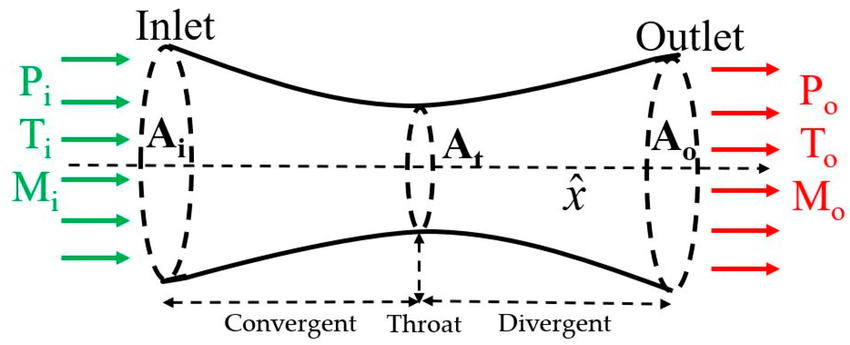
\includegraphics[width=0.5\linewidth]{images/de-laval-nozzle.png}
    \caption{Clasical De Laval Nozzle}
    \label{fig:placeholder}
\end{figure}

The aerospike nozzle, by contrast, automatically adapts to a wider range of atmospheric pressures thanks to the \href{https://en.wikipedia.org/wiki/Prandtl–Meyer_expansion_fan}{Prantl-Meyer expansion fan}. This makes it especially attractive for single-stage-to-orbit (SSTO) vehicles, which must operate efficiently from sea level to vacuum. Aerospike nozzles can also achieve very high expansion ratios with less structural mass.

\begin{figure}[H]
    \centering
    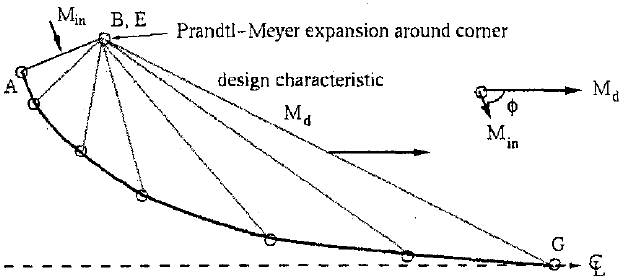
\includegraphics[width=0.5\linewidth]{images/prantl-meyer-expansion.png}
    \caption{Prantlt Meyer Expansion}
    \label{fig:pr-mey}
\end{figure}

However, aerospike nozzles are notoriously difficult to cool, particularly as engine size increases. This is a classic example of scaling effects, sometimes summarized by the saying ``an elephant is not simply a large mouse, and a mouse is not simply a small elephant.'' In engineering, many systems do not scale linearly, and designs that work well at one size may become impractical at another.

\subsection{Current Recipe}

At present, rocket engines are designed using the \textit{Rocket Engineer Table}.

\begin{figure}[H]
    \centering
    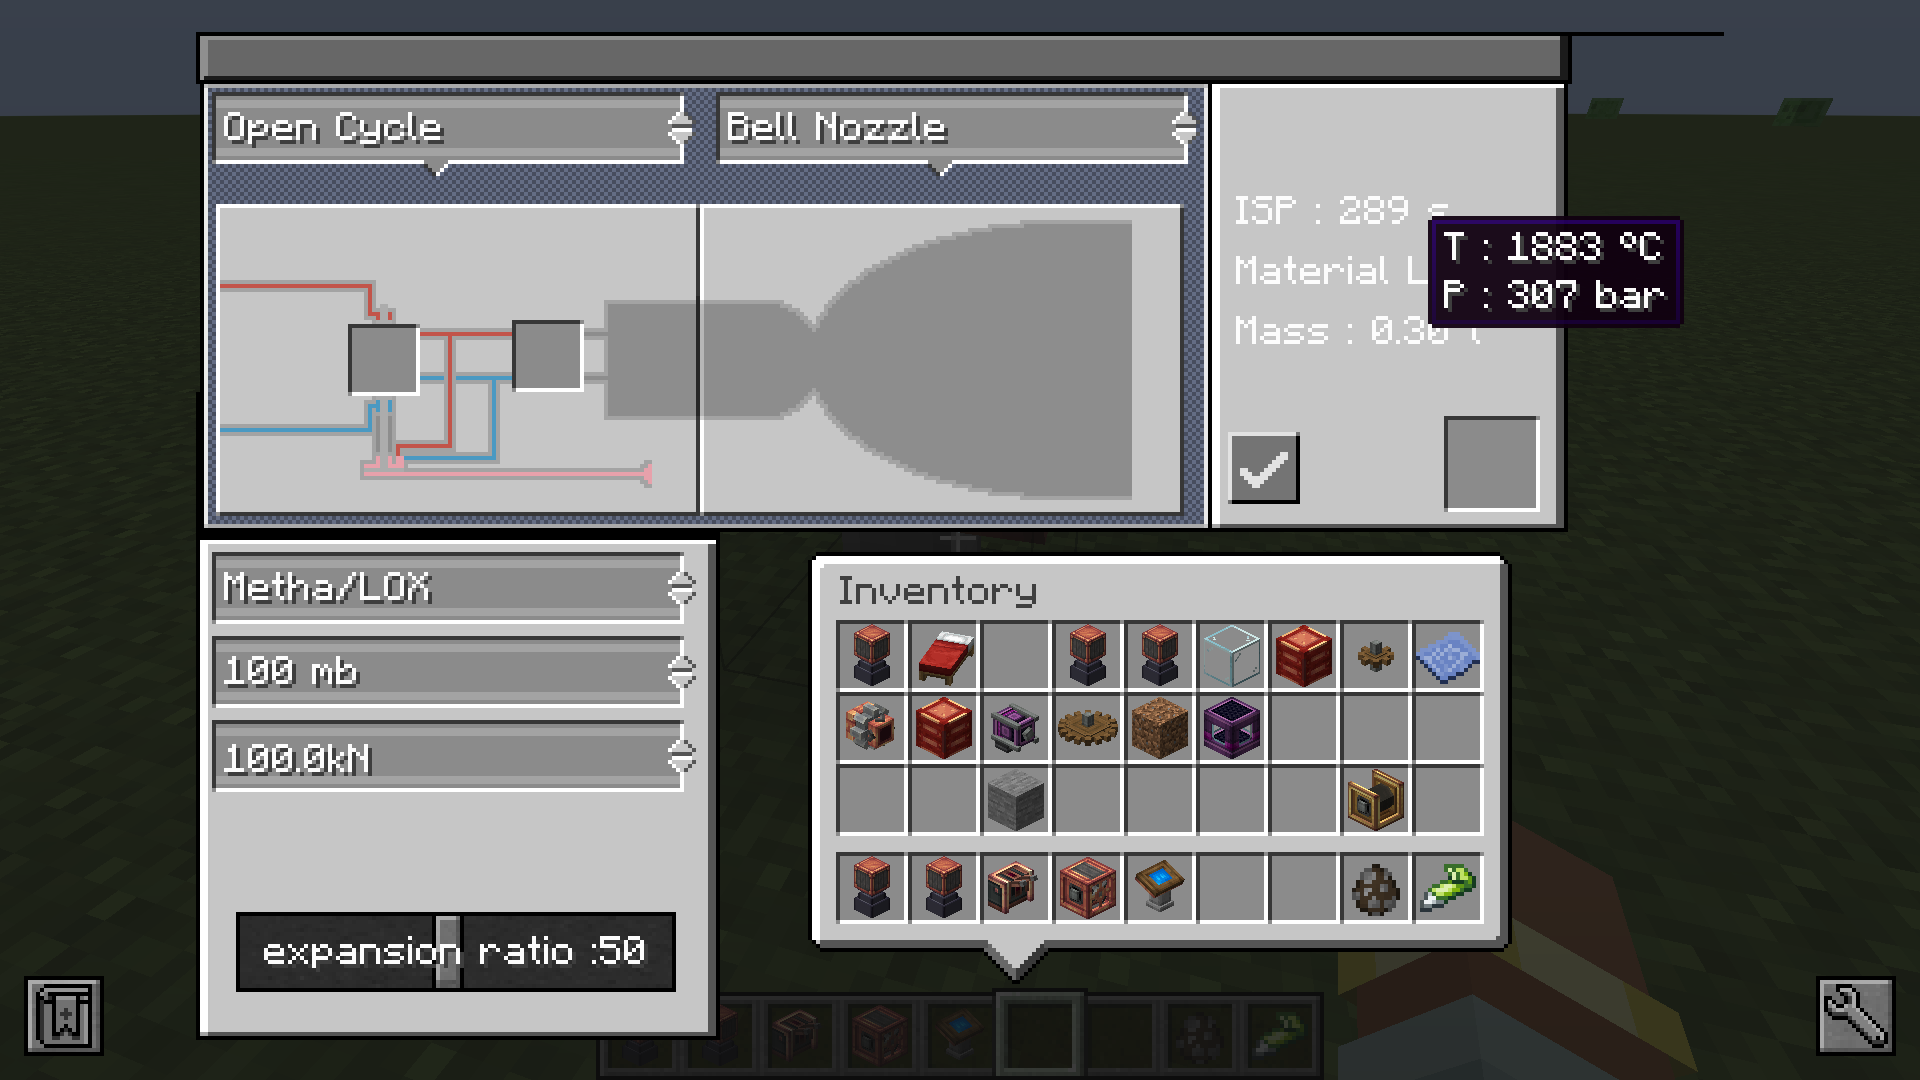
\includegraphics[width=0.75\linewidth]{images/engineer_table_1.png}
    \caption{Rocket Engineer Table}
    \label{fig:rocket_engineer_table}
\end{figure}

The interface contains six selectors, arranged from top to bottom and left to right.

The first selector is the \textit{power pack}. It defines the technology used to pump and burn the propellants, including the turbopumps, the plumbing layout, and the injectors. These parameters determine how efficiently the propellants are mixed and the effective size of the combustion chamber.

The second selector is the \textit{exhaust pack}, which determines how the combustion gases are expanded and accelerated to generate thrust.

The third selector specifies the \textit{propellant combination}, that is, the fuels and oxidizers used and their mixture ratio.

The fourth selector sets the \textit{combustion chamber volume}. The throat area is directly proportional to this value.

The fifth selector defines the \textit{target thrust}.

Finally, the sixth selector controls the \textit{expansion ratio}.

The panel on the left displays the resulting engine characteristics:

\begin{itemize}
    \item Specific impulse (ISP), which represents engine efficiency.
    \item Material level, determined by the chamber temperature and pressure requirements.
    \item Engine mass.
    \item Chamber temperature (shown in a tooltip).
    \item Chamber pressure (shown in a tooltip).
\end{itemize}

The material level is computed by applying separate penalties based on chamber pressure and temperature. The required material corresponds to the addition of the two penalties. This approach allows both thermal resistance and mechanical strength to influence material selection.

\begin{table}[H]
    \centering
    \caption{Material level penalties based on operating conditions}
    \label{tab:material-penalties}
    \begin{tabular}{|c|l|l|}
        \hline
        \textbf{Level Penalty} & \textbf{Pressure Range} & \textbf{Temperature Range} \\
        \hline
        0 & $< 3$ bar & $< 300\,^\circ$C \\
        1 & 3 -- 50 bar & 300 -- 1\,000 $^\circ$C \\
        2 & 50 -- 200 bar & 1\,000 -- 2\,000 $^\circ$C \\
        3 & 200 -- 1\,000 bar & 2\,000 -- 5\,000 $^\circ$C \\
        4 & $> 1\,000$ bar & $> 5\,000\,^\circ$C \\
        \hline
    \end{tabular}
\end{table}

The resulting material progression is shown in Table~\ref{tab:material-progression}.

\begin{table}[H]
    \centering
    \caption{Material progression and alloy recipes}
    \label{tab:material-progression}
    \begin{tabular}{|c|l|l|}
        \hline
        \textbf{Level} & \textbf{Material} & \textbf{Recipe} \\
        \hline
        0 & Andesite & Built-in \\
        1 & Iron & Built-in \\
        2 & Copper & Built-in \\
        3 & Brass & Built-in \\
        4 & Reinforced Copper (Cu--Fe) & 2 Cu + 1 Fe $\rightarrow$ 3 \\
        5 & Cupronickel (Copper--Nickel) & 2 Cu + 1 Ni $\rightarrow$ 3 \\
        6 & Monel (Nickel--Copper) & 2 Ni + 1 Cu $\rightarrow$ 1 \\
        7 & Inconel (Nickel--Iron) & 2 Ni + 1 Fe $\rightarrow$ 1 \\
        8 & Hastelloy (Ni--Co--Cu--Fe) & 2 Ni + 2 Co + 1 Cu + 1 Fe $\rightarrow$ 2 \\
        \hline
    \end{tabular}
\end{table}

\subsection{Issues, Bugs, and Sources of Confusion}

The material level is determined solely by the chamber temperature and pressure. However, the thresholds are not well balanced, allowing extremely high chamber pressures to be reached at relatively low cost. This reduces the importance of material progression and leads to unrealistic designs.

Crafting is also highly repetitive. Most engine components are produced through nearly identical sequenced assembly recipes that differ only in the material used. In addition, each engine is built entirely from a single material, which is both unrealistic and limits design variety.

The number of available alloys is arguably too high, and many of them have very similar recipes and properties. This makes progression harder to understand without adding significant gameplay depth.

Lastly one of the visual issue is that the rocket engine model is allways the same, whatever the exhaust and power pack may be, it would be nice to have a few different variation, in particular in the number of turbopumps for the power pack and the aspect of the nozzle bwn a aerospike and a bell nozzle. Additionaly it would be nice to scale it with the chamber volume.




\subsection{Possible Improvements}

One way to make the system more approachable for casual players would be to provide pre-designed engine blueprints as dungeon loot or progression rewards. Players who are not interested in detailed engineering could use these proven designs directly, while more advanced players could modify and optimize them.

Materials should have clearly defined limits for both temperature and pressure. An even more realistic approach would be to make the maximum allowable pressure depend on temperature. This would allow materials to be balanced more accurately and would create more meaningful engineering trade-offs. An make either chose the lowest material level that could fit for a given temperature, or chose a material and allowing the recipe if it's within bounds and show how much margin you have : like currentP/maxP and currentT/maxT.

%%in futur put an image to illustrate both choices

The Rocket Engineer Table could also be replaced with a nodal computation interface, similar to the piston engine simulation shown below.

\begin{figure}[H]
    \centering
    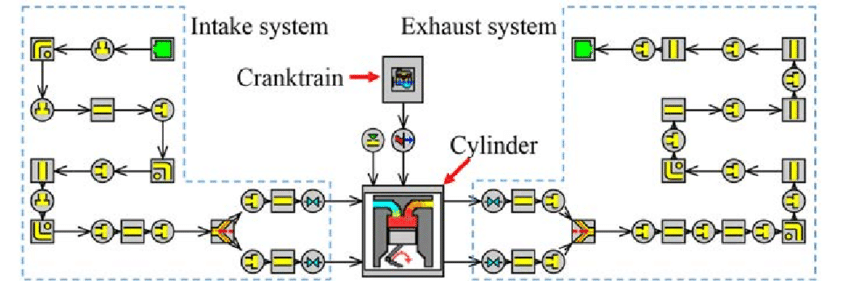
\includegraphics[width=0.75\linewidth]{images/nodal_simulation_exemple.png}
    \label{fig:nodal_simulation_example}
\end{figure}

Such a system would allow players to build engines by connecting functional components visually. Implementing this would require draggable widgets, a design saving system, automatic fluid assignment for propellants, and a component-linking mechanism. This approach would fit well with the blueprint concept: beginners could rely on pre-made examples, while advanced players would gain access to a much deeper and more engaging design process.

The number of alloys could also be reduced. Andesite, Copronickel, Reinforced Copper, and at least one of the high-performance superalloys could potentially be removed without significantly affecting progression.

Finally, all engine components should be recyclable in order to reduce material waste and encourage experimentation.

\section{Spacesuit}

The current spacesuit has 2 version : the basic crafted with copper and the advanced crafted with netherite.
It has a few major issues :
First the refilling of the backtank require taking it off and placing it on the ground, having 2 seperate oxygen bottles either refiled with the spout or a new processing machine.
Second the armor is fixe it should be able to recive armor upgrades especialy if you have modpacks that introduce strnger than netherite materials.
Third it should be able to provide air pressure for create tool like the extendo grip.
Forth, helytras shouldn't work in space, make a jetpack slot too manuver in 0g and move faster on other planets.
Magentic boots to avoid floating in 0g, Corosion resistance. (maybe as an enchantements, but make sure it is easy enough to get to not being anoying)
Harpon ?

\begin{figure}[H]
    \centering
    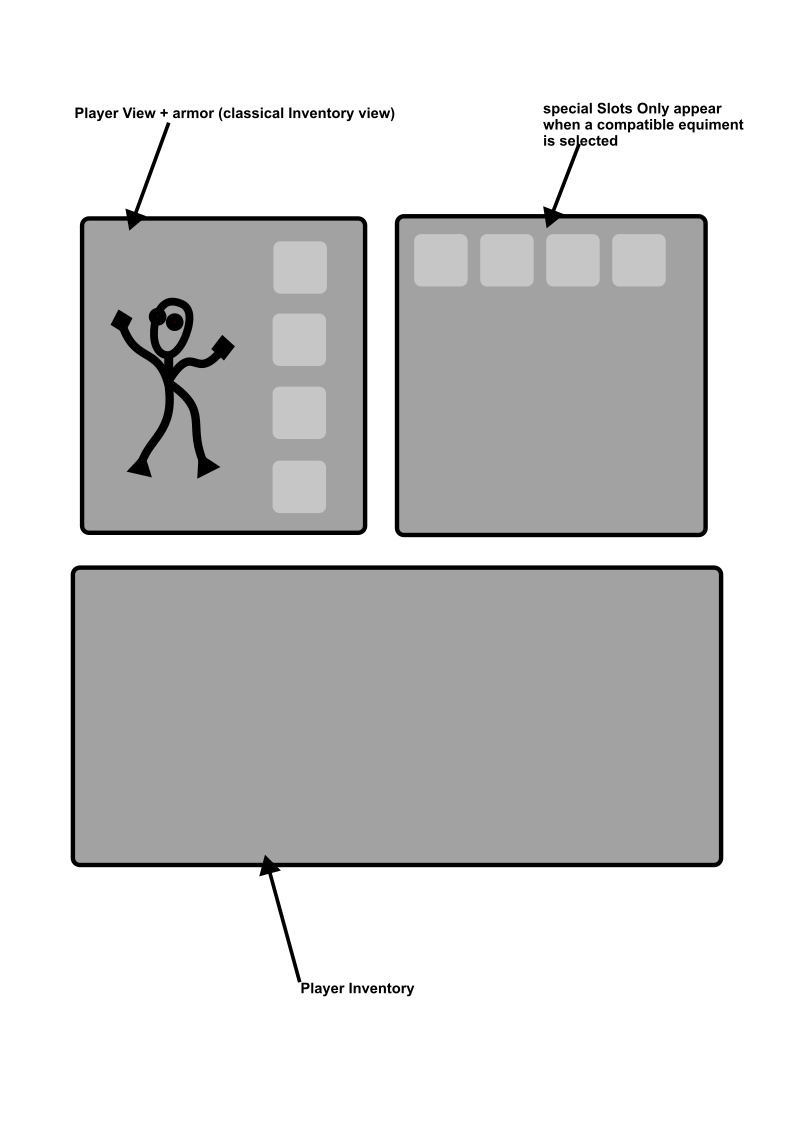
\includegraphics[width=0.75\linewidth]{images/new_armor_menu.png}
    \caption{Futur Spacesuit menu}
    \label{fig:futur_spacesuit}
\end{figure}

\section{Sealed Atmosphere}

\subsection{Current State}

Sealers are used to pressurize enclosed rooms. They are implemented as non-intersecting axis-aligned bounding boxes (AABBs) that define sealed volumes. These volumes are recomputed whenever a block state change is detected inside the sealed area.

\subsection{What to Improve}

Future improvements aim to make the sealed atmosphere system more visually and mechanically consistent. Planned additions include atmospheric effects and particle systems that appear at leak points, allowing players to visually detect pressure loss.

A more advanced gas simulation is also planned. This includes introducing multiple gas types such as oxygen and carbon dioxide, rather than relying solely on oxygen partial pressure. This would enable systems such as air recycling, CO$_2$ buildup, and life-support management.
Change the storage system to be able to rebuild without dropping everything.
etither with an octogrid, or with a binary tree of AABBs (it's either a leaf, or contains 2 childs that are strictly contained, in the sense that the parent is the minimum containg AABB)

\section{Planets Definition}

\subsection{Gravity}



\subsection{Adjacency Map}

Planets are planned to be connected through an adjacency map, where each connection represents the required $\Delta v$ to travel between two celestial bodies. This creates a directed graph of travel costs that can be used for navigation planning, automation, and progression balancing.

\subsection{Atmosphere Configuration}

Atmosphere configuration is not yet implemented. The goal is to define each planet's atmospheric composition and pressure, which can then be used to derive gameplay-relevant properties such as fog density, visibility distance, and environmental hazards.

In particular, atmospheric pressure will influence the maximum fog density and rendering distance, creating distinct visual identities for each planet.

For reference and inspiration on atmospheric scattering and fog behavior, see:
https://www.youtube.com/watch?v=DxfEbulyFcY

\subsection{Planetarium}
Who, orbits, who and the orbital parameters. This will give the time of day and the place of each body in the sky. It also means that the time of day is out of sync in bwn planets and sleeping can introduce weird issues in multiplayers.

\section{World Generation}

\subsection{World Generation System Presentation}

Minecraft uses a sophisticated world generation system based on \textit{density functions}, which are mathematical expressions evaluated at every point in the world. These functions determine whether a given location is solid or empty and therefore define the shape of terrain, caves, and underground structures. Since Minecraft 1.18, nearly all world generation parameters have been defined through datapacks, making the system highly customizable.

For each dimension, three main datapack entries are required:

\begin{itemize}
    \item The \textit{dimension} definition, which specifies the dimension type and the biome source.
    \item The \textit{dimension type}, which controls environmental properties such as world height, coordinate scaling, lighting, and sky effects.
    \item The \textit{noise settings}, which define the terrain generation process and reference the density functions used to shape the landscape.
\end{itemize}

Together, these three files determine both the appearance and the physical properties of a dimension.

\subsubsection{Density Functions}

Density functions are the mathematical core of Minecraft's terrain generation. They combine procedural noise, arithmetic operations, interpolation, and conditional expressions to compute scalar values at each coordinate in the world.

These functions are used not only to determine whether a block is solid or empty, but also to generate the climate parameters that drive biome placement.

Minecraft provides a large set of built-in density function types, including constants, arithmetic combinations, clamping, interpolation, and several noise samplers based on Perlin-derived algorithms. Some functions operate in three dimensions, while others effectively ignore one or more coordinates to create two-dimensional maps.

Creating Space extends this system by introducing additional function types, including Worley noise and erosion maps based on the Phacelia erosion technique. This method produces procedural erosion patterns that mimic the large-scale effects of hydraulic and thermal erosion while remaining efficient enough to be evaluated during world generation. These additions make it possible to generate more realistic asteroid and heavily eroded planetary surfaces.

\subsubsection{Noise Settings}

The noise settings file defines how terrain is generated within a dimension. It specifies parameters such as the minimum Y level, total world height, sea level, default blocks and fluids, and the \textit{noise router}.

The noise router is a collection of density functions used by different parts of the terrain generator. Its main components include:

\begin{itemize}
    \item Aquifer functions: \texttt{initial\_density\_without\_jaggedness}, \texttt{barrier}, \texttt{fluid\_level\_floodedness}, \texttt{fluid\_level\_spread}, and \texttt{lava}. These functions determine where underground water and lava are placed.
    \item Climate functions: \texttt{temperature}, \texttt{vegetation}, \texttt{continents}, \texttt{erosion}, \texttt{depth}, and \texttt{ridges}, which are passed to the biome source.
    \item Terrain shaping functions, most importantly \texttt{final\_density}, which determines whether each block position is solid or empty.
    \item Ore vein functions such as \texttt{vein\_toggle}, \texttt{vein\_ridged}, and \texttt{vein\_gap}, used to generate large iron and copper ore deposits.
    \item Surface rules, which replace the top layers of terrain with biome-appropriate blocks such as grass, sand, regolith, or ice.
\end{itemize}

By modifying these settings, it is possible to create a wide variety of planetary landscapes.

\subsubsection{Dimension and Biome Source}

The dimension definition links together the dimension type and the biome source.

The biome source determines which biomes are placed at each location. The most common implementation is the \texttt{multi\_noise} biome source, which selects biomes according to six climate parameters: temperature, vegetation (also called humidity), continentalness, erosion, depth, and weirdness (also called ridges).

One of the strengths of this system is that biome placement can follow terrain features. This is particularly visible with the \texttt{depth} parameter, which is derived from a terrain estimate without caves and can therefore distinguish between underground, surface, and elevated regions. In Creating Space, these climate parameters are not necessarily interpreted as Earth-like climate variables; THEY CAN BE REASSIGNED to represent any planetary property relevant to biome distribution.

In Creating Space, these systems are used extensively to generate planets and moons with unique terrain, climates, and visual characteristics while relying almost entirely on Minecraft's native datapack-based world generation framework.


\subsection{Venus}

Venus is designed as a hostile volcanic world dominated by dense clouds, toxic lowlands, and extensive cave systems. Its biome distribution is relatively simple but creates strong visual contrasts between high volcanic terrain and corrosive basins.

\subsubsection{Existing Biomes}

Venus currently contains four biomes:

\begin{itemize}
    \item \textbf{Volcano}: Chaotic and montain terrain (\texttt{continentalness} from 0.3 to 1.0) representing ancient volcanic regions and shield volcanoes.
    \item \textbf{Toxic}: river filled plain (\texttt{continentalness} from -1.0 to -0.2) with high humidity values, representing chemically active areas with dense toxic deposits.
    \item \textbf{Plain}: The most common surface biome, very flat
    \item \textbf{Cave}: Underground biome generated beneath volcanic regions.
\end{itemize}

The current parameter assignment uses \texttt{continentalness} to distinguish high volcanic terrain from flatter plains, while \texttt{humidity} separates toxic regions from normal plains.

\subsubsection{Existing Structures}

No structures have been implemented yet.

\subsubsection{Work Remaining}

\begin{itemize}
    \item Polish the world generation, especially cave generation and aquifer behavior.
    \item Rework the Toxic biome, including both textures and environmental features.
    \item Add Venus-specific mobs adapted to the extreme environment.
    \item Introduce structures such as abandoned probes, automated factories, high altitude cities.
    \item add erosion to the volcanoes, add magma chamber to them and use 2d worley instead of 3d in addition to the interpolation to make the worldgen faster.
\end{itemize}


\subsection{Moon}

The Moon is intended to provide an early/mid-game extraterrestrial destination. Its terrain focuses on cratered plains, mountains, and underground facilities.

\subsubsection{Existing Biomes}

The Moon currently contains three biomes:

\begin{itemize}
    \item \textbf{Plains}: Broad regolith-covered lowlands.
    \item \textbf{Mountains}: Elevated and rugged terrain.
    \item \textbf{Cave}: Underground lava tubes and subsurface voids.
\end{itemize}

Large impact craters are generated independently of biome placement and form one of the defining features of the lunar surface.

\subsubsection{Existing Structures}

Several structures are already implemented or in development:

\begin{itemize}
    \item \textbf{Outpost}: A small exploration base.
    \item \textbf{Underground Base}: Currently under development.
    \item \textbf{Crashed Ships}: Wrecked spacecraft, also under development.
\end{itemize}

\subsubsection{Work Remaining}

\begin{itemize}
    \item Complete texture integration and visual polishing.
    \item Improve crater generation by reducing crater density and integrating craters more naturally into the surrounding terrain.
    \item Investigate a noise-based approach for large craters using two-dimensional Worley noise.
    \item Remove the obsolete crashed rocket structure.
    \item Expand loot tables.
    \item Add cave features such as ice spikes.
    \item Introduce lunar mobs if appropriate.
\end{itemize}


\subsection{Mars}

This section describes the Mars dimension, including its biome distribution, planned structures, and remaining development tasks. Mars uses the 6-dimensional multi-noise biome system, where each biome is defined through a combination of temperature, humidity, erosion, continentalness, weirdness, and depth parameters.

\subsubsection{Existing Biomes}

Mars is generated using a multi-noise biome system where each biome is defined by ranges across six parameters. These parameters control both large-scale terrain generation and biome placement.

The main parameter meanings are adapted to the Martian context:

\begin{itemize}
    \item \textbf{Temperature}: Used primarily to control ravine presence and extreme terrain features.
    \item \textbf{Humidity}: Represents moisture availability and is used for mossy or water-related biomes.
    \item \textbf{Erosion}: Controls surface roughness and transition between smooth and fractured terrain.
    \item \textbf{Continentalness}: Represents elevation, from deep basins to high mountain regions.
    \item \textbf{Weirdness}: Controls terrain variation, including hills, ridges, and large-scale distortions.
    \item \textbf{Depth}: Distinguishes surface terrain from underground cave systems.
\end{itemize}

The Martian surface is divided into the following biome families:

\paragraph{Surface Biomes (depth: -1 to 0.2)}

\begin{itemize}
    \item \textbf{Plains}: The most common biome, occurring in lowlands and moderate elevations. Includes both flat plains and elevated plains depending on continentalness.
        \begin{figure}[H]
            \centering
            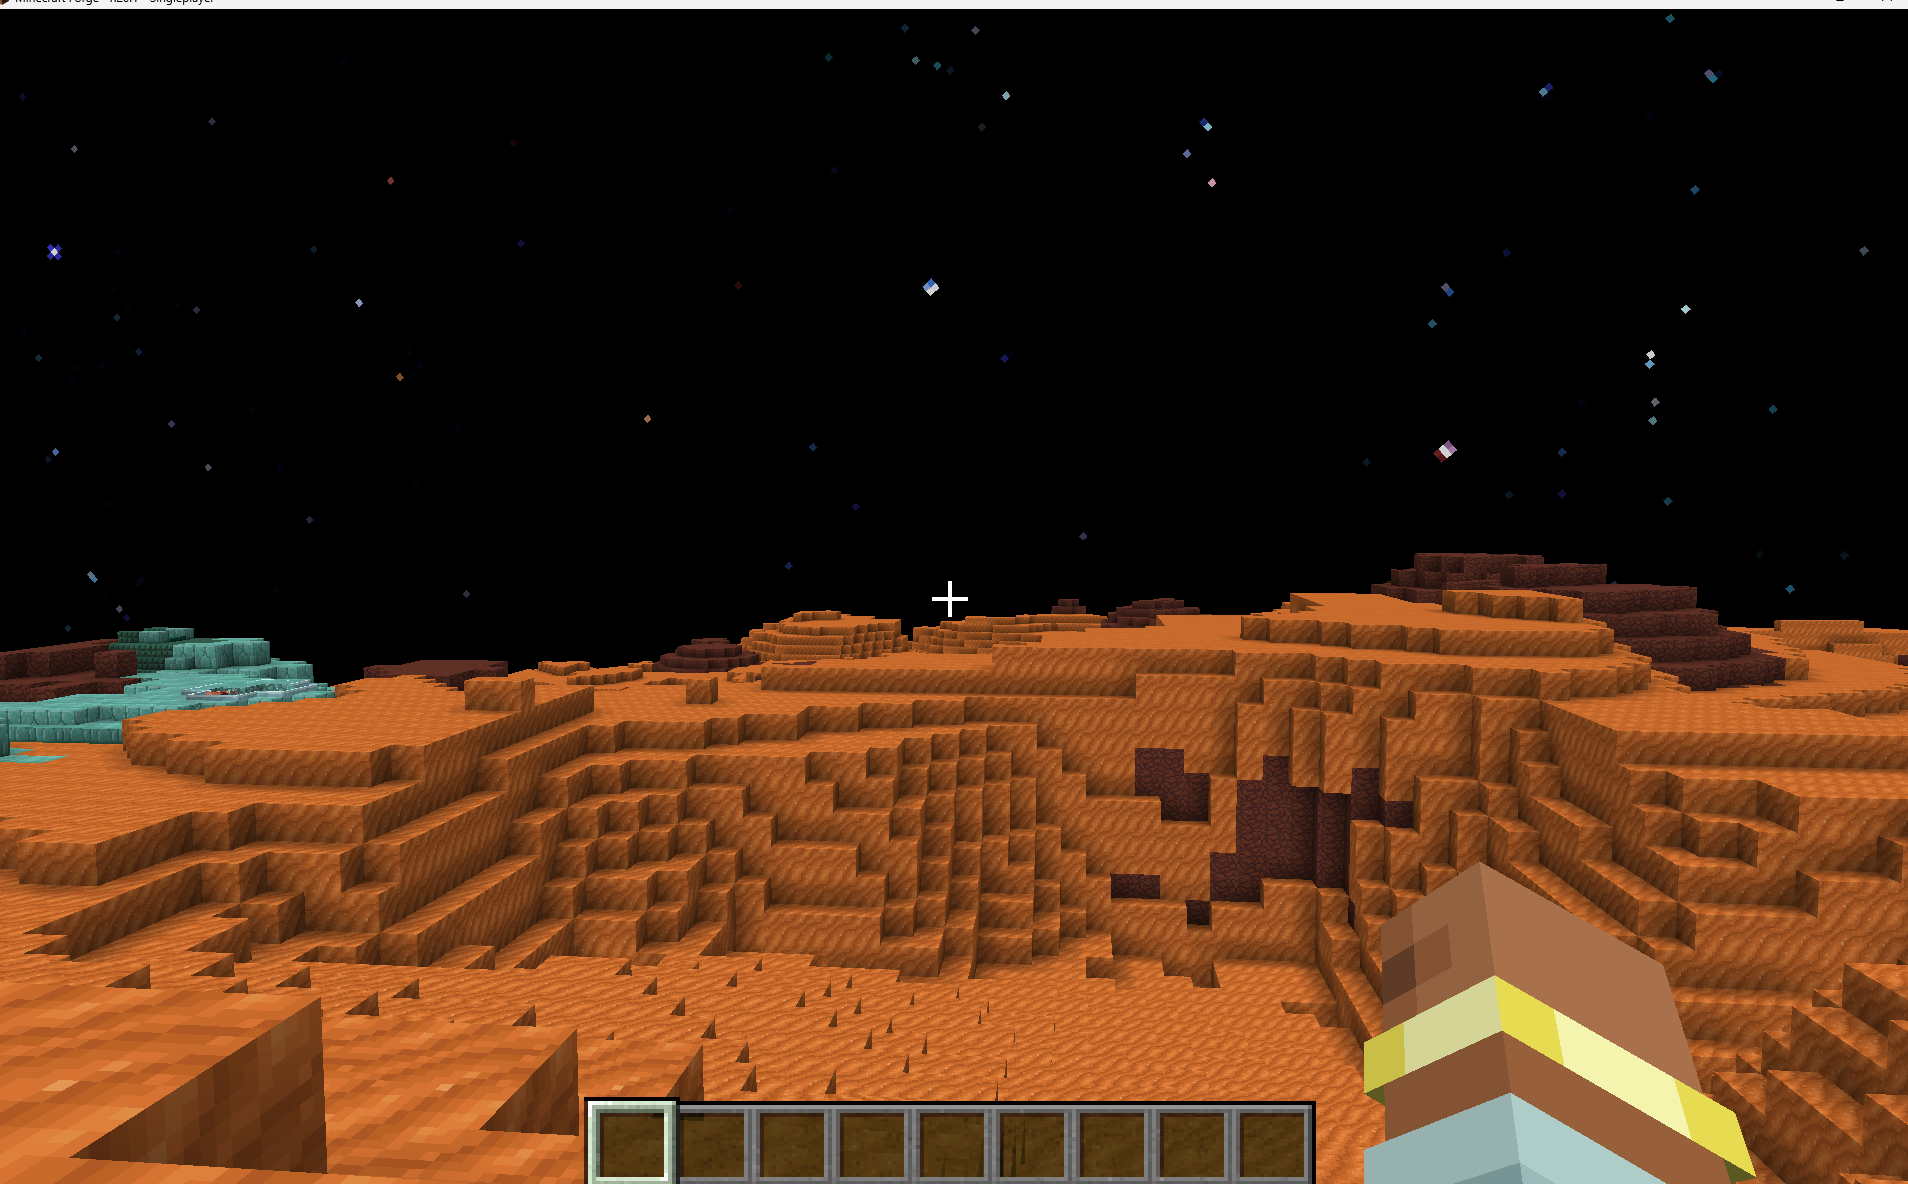
\includegraphics[width=0.75\linewidth]{images/flat_plain.png}
            \label{fig:mars-flat-plain}
        \end{figure}
        \begin{figure}[H]
            \centering
            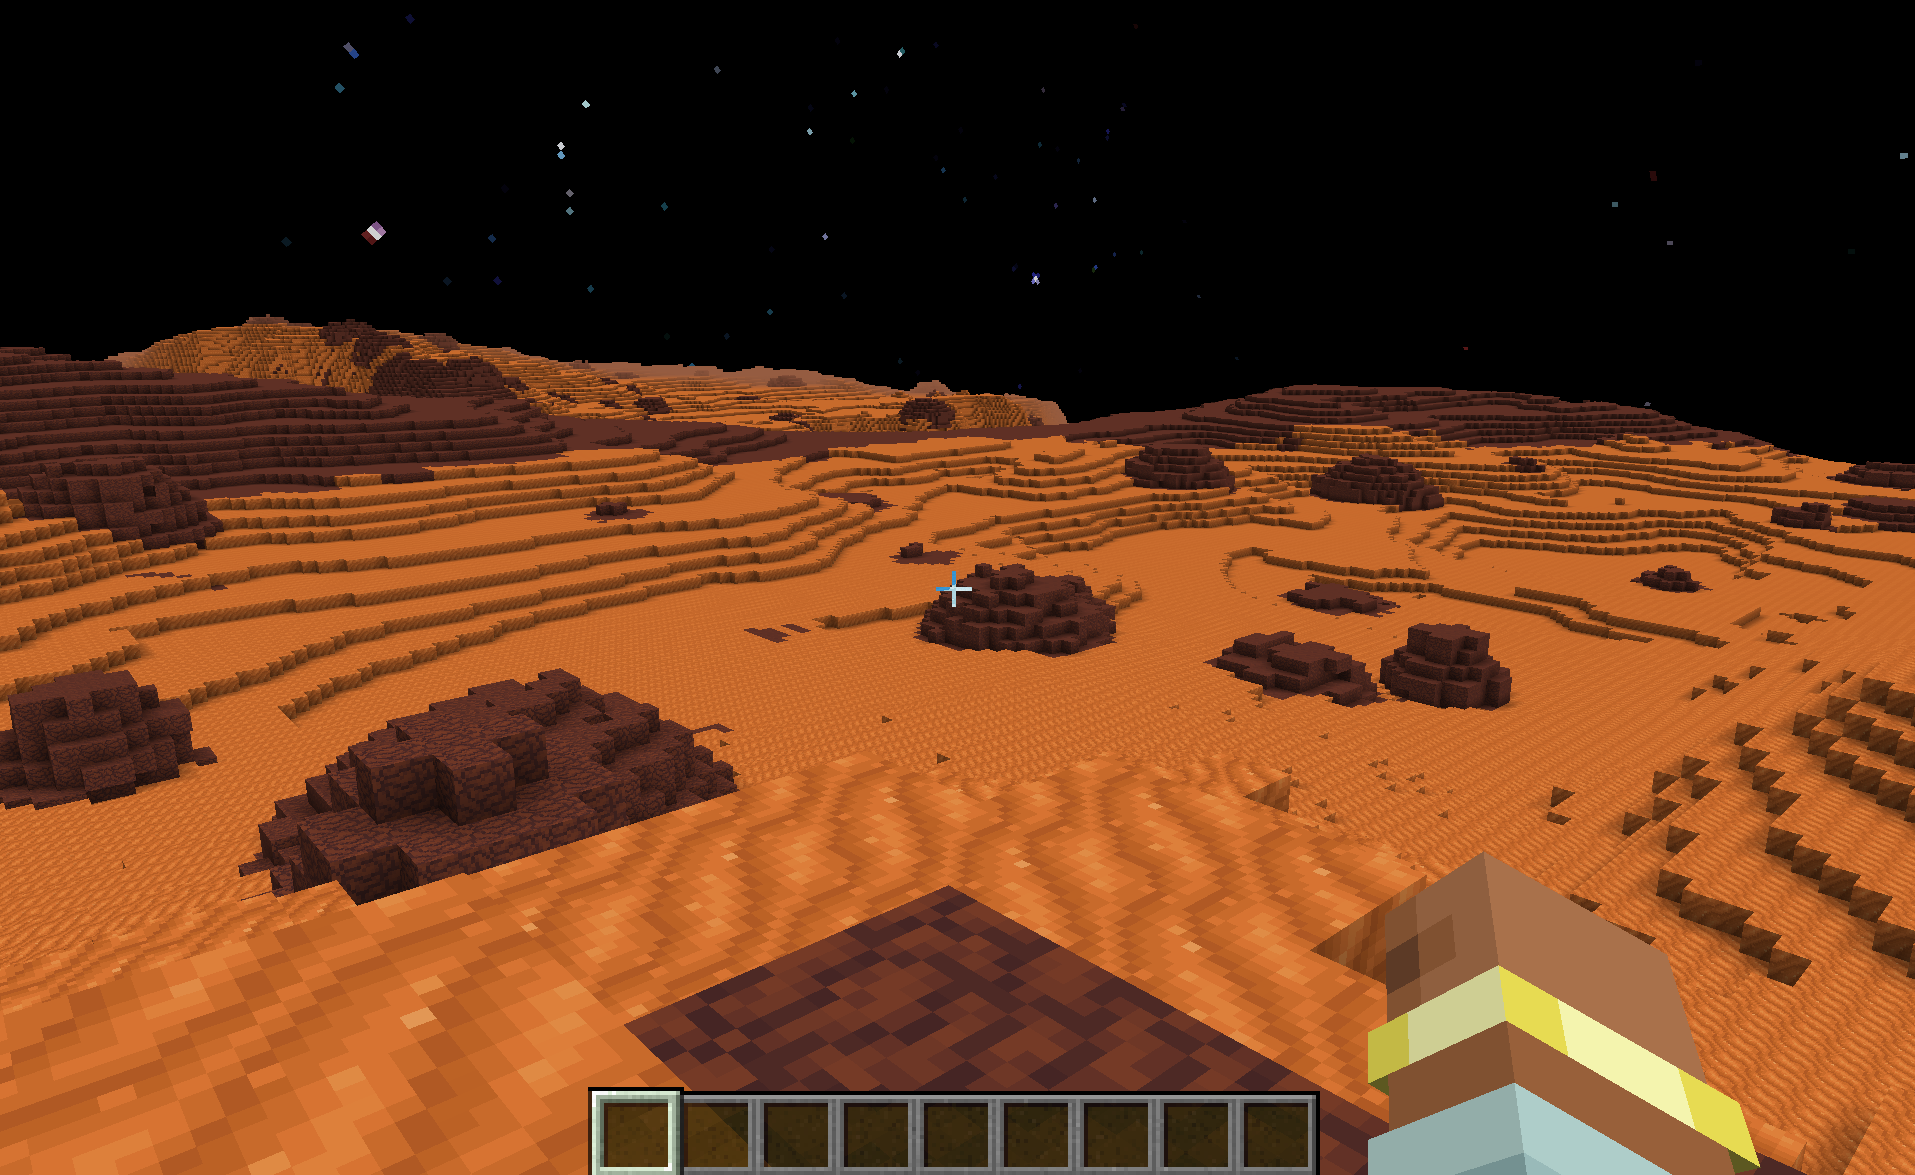
\includegraphics[width=0.75\linewidth]{images/elevated_plain.png}
            \label{fig:mars-elevated-plain}
        \end{figure}
    \item \textbf{Mountains}: High elevation terrain with strong variation in weirdness, producing rugged rocky formations.
        \begin{figure}[H]
            \centering
            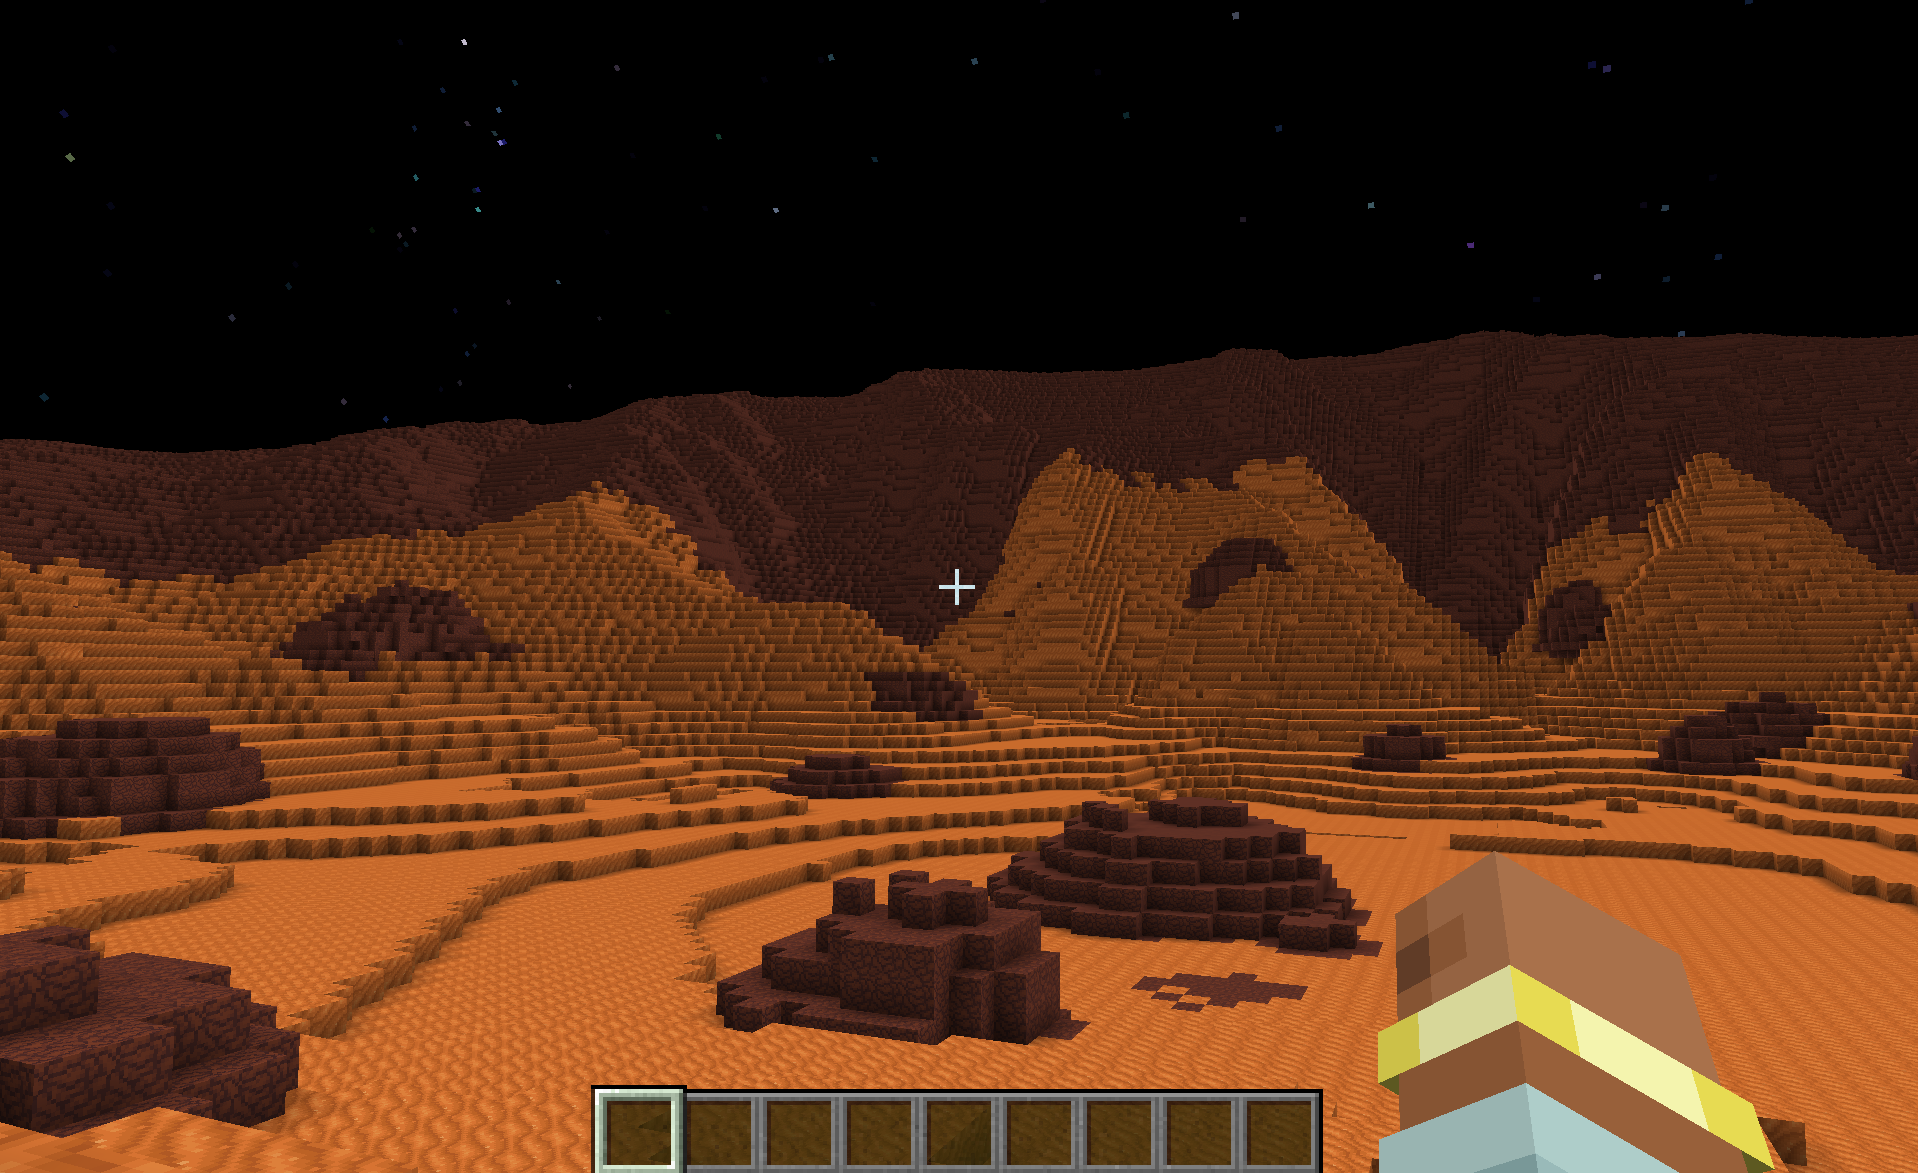
\includegraphics[width=0.75\linewidth]{images/montain.png}
            \label{fig:mars-mountains}
        \end{figure}
    \item \textbf{Ocean}: Low-lying basins representing ancient Martian lakes or seas.
        \begin{figure}[H]
            \centering
            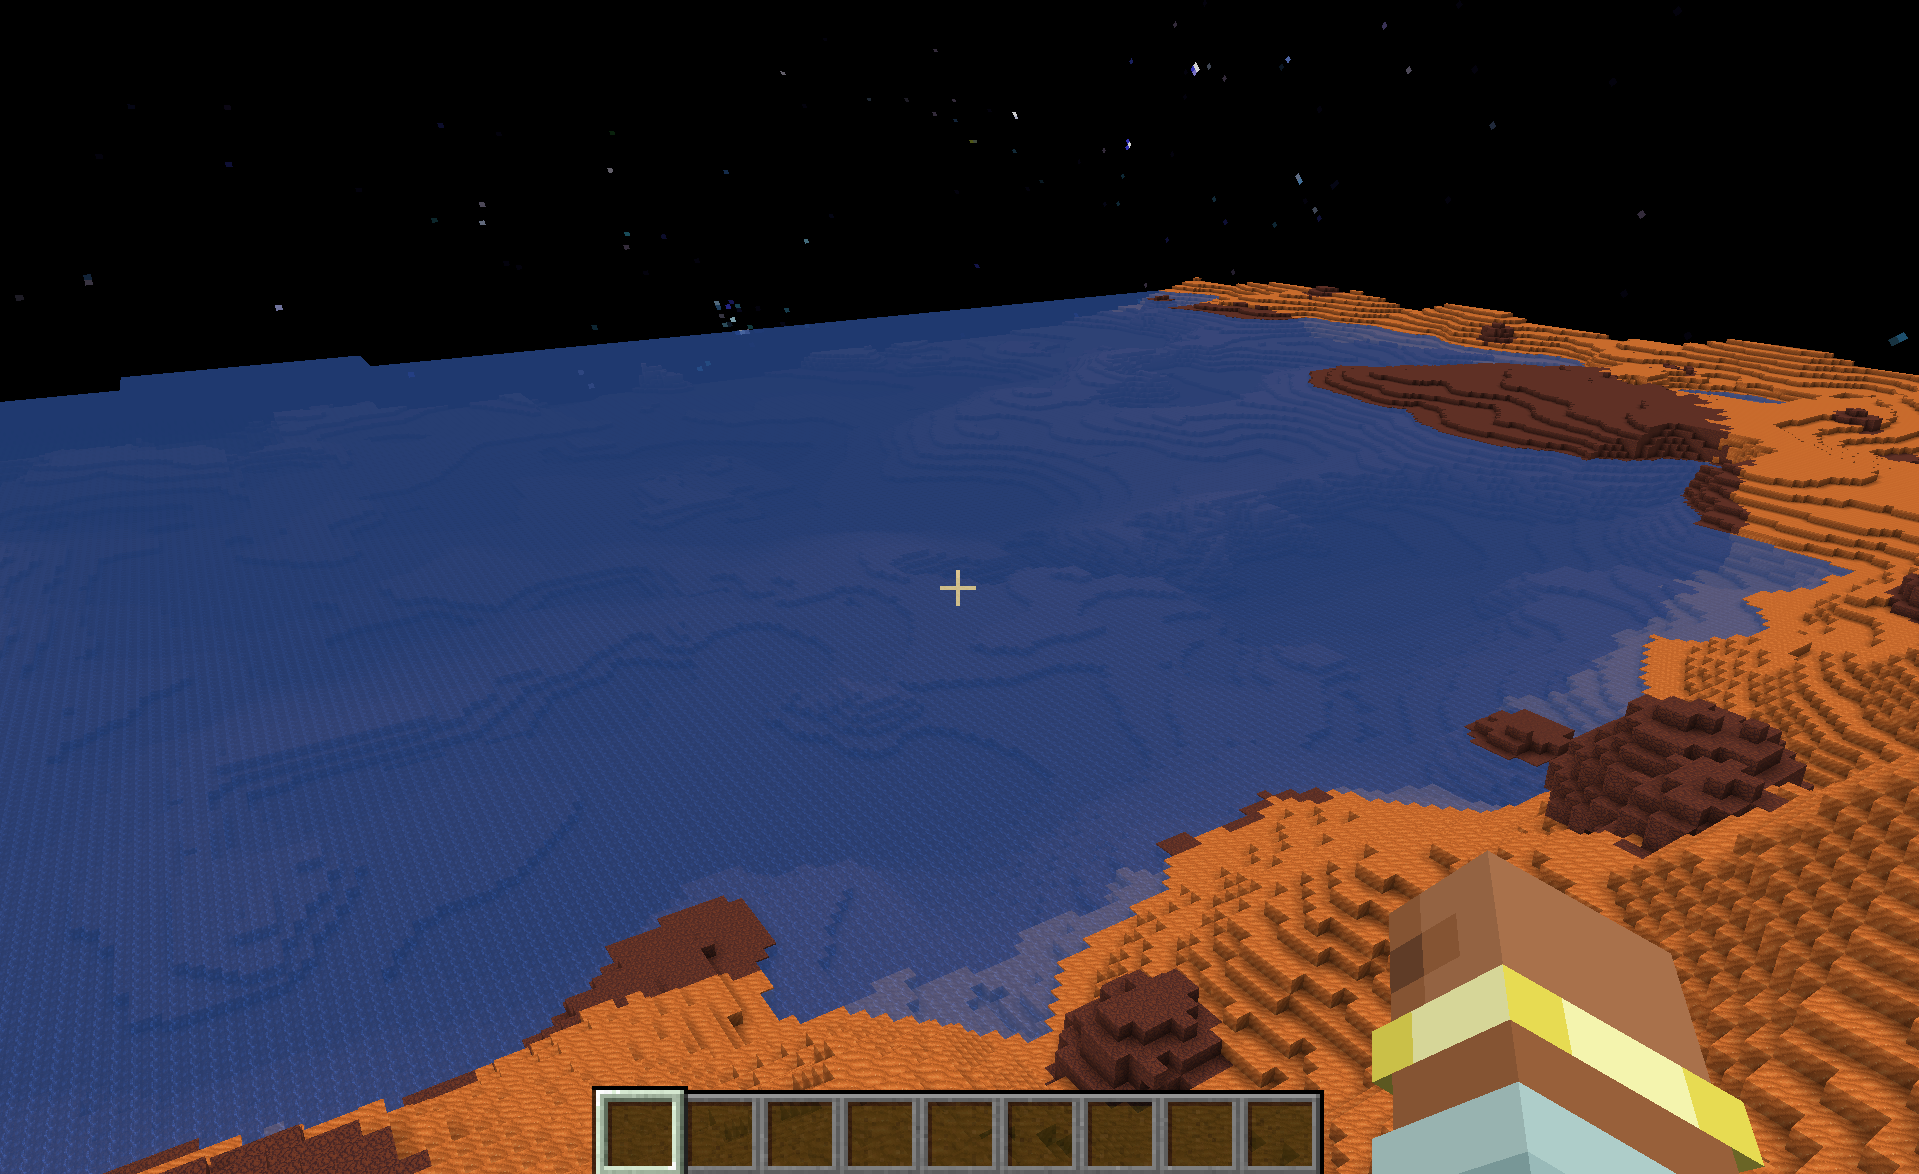
\includegraphics[width=0.75\linewidth]{images/ocean.png}
            \label{fig:mars-ocean}
        \end{figure}

    \item \textbf{Mossy Ravine Variants}: Rare moisture-rich regions characterized by ravine structures and vegetation. These include:
    \begin{itemize}
        \item Mossy Ravine Forest (high moisture)
        \item Mossy Ravine (moderate moisture)
    \end{itemize}
    \begin{figure}[H]
        \centering
        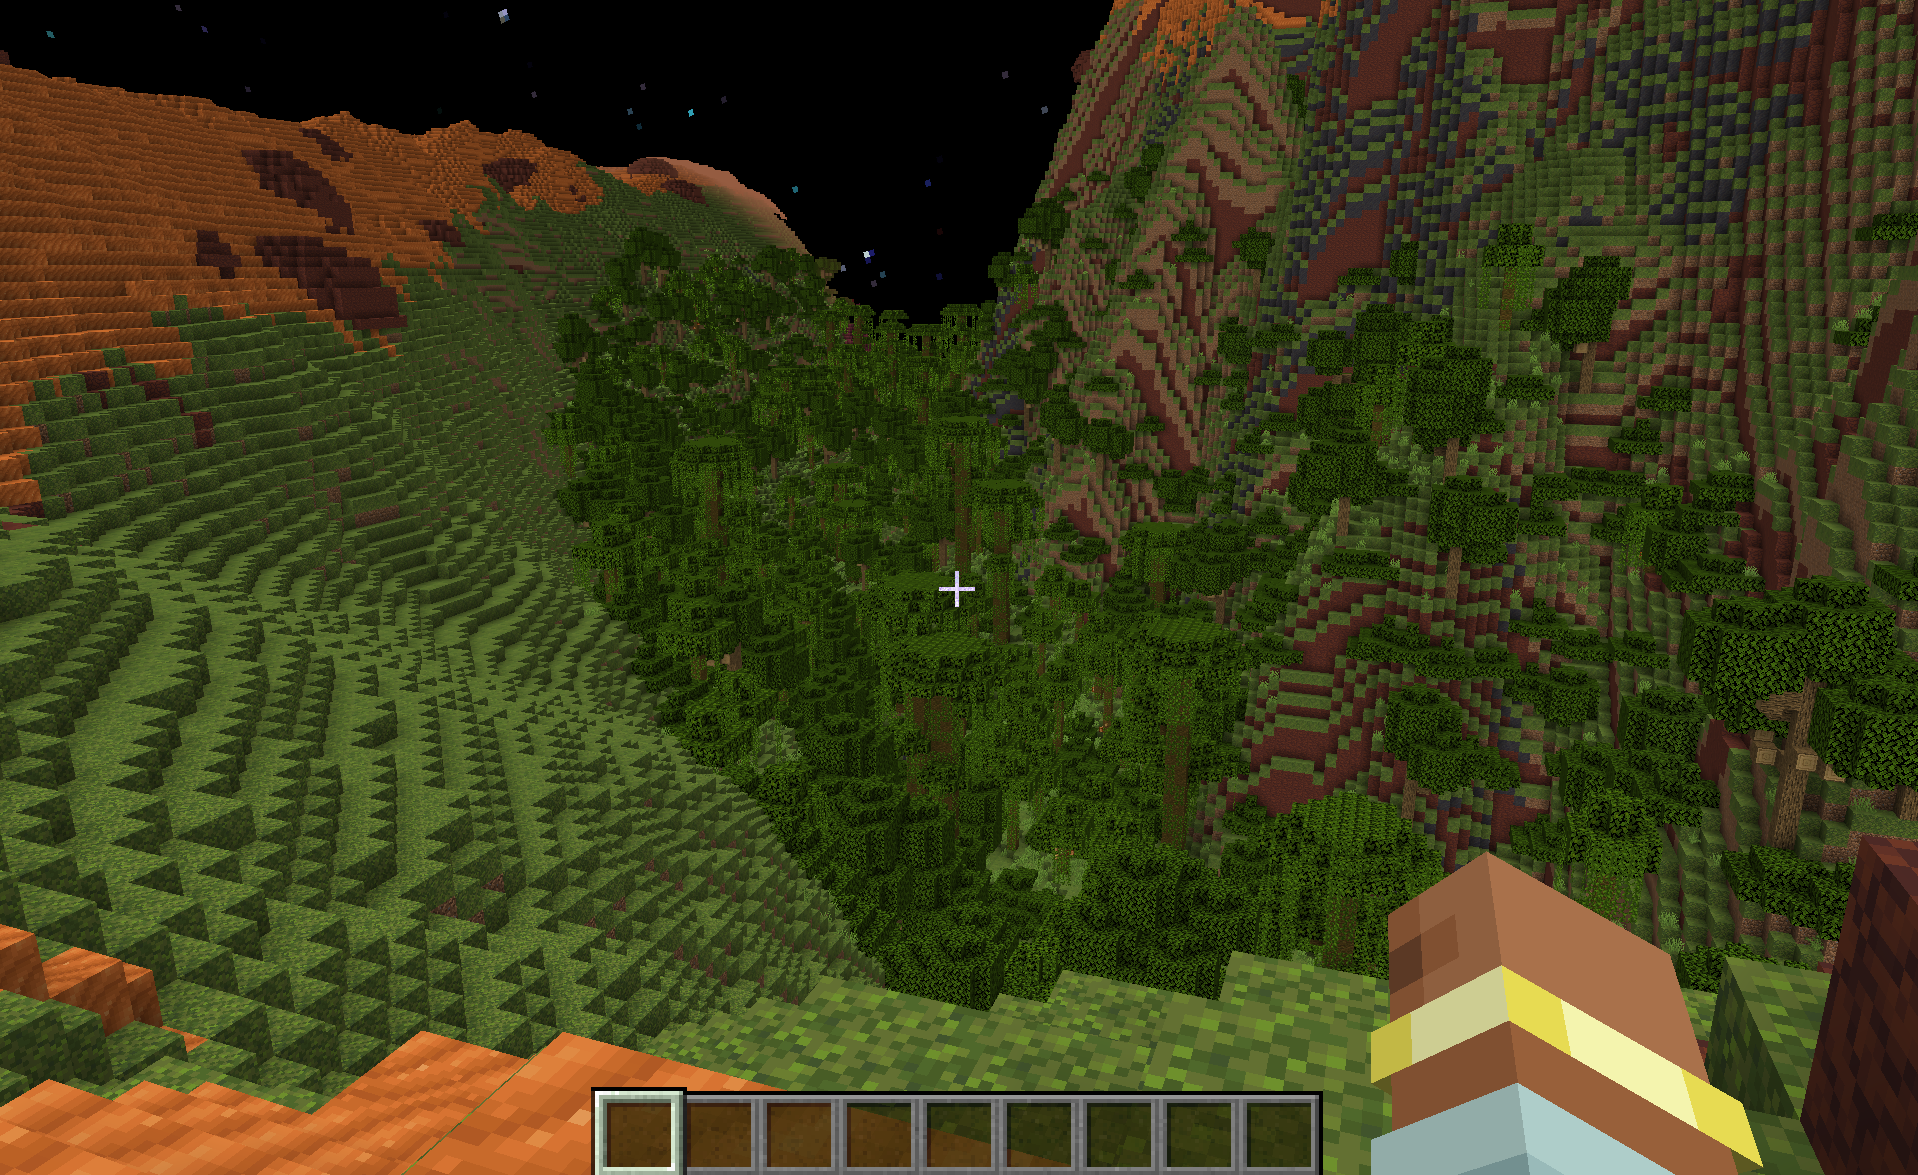
\includegraphics[width=0.75\linewidth]{images/mossy_ravine.png}
        \label{fig:mars-mossy-ravine}
    \end{figure}
\end{itemize}


\paragraph{Underground Biomes (depth: 0.1 to 1)}

\begin{itemize}
    \item \textbf{Cave}: A universal underground biome generating below the surface. It includes cave systems, tunnels, and subsurface voids.
\end{itemize}

\begin{figure}[H]
    \centering
    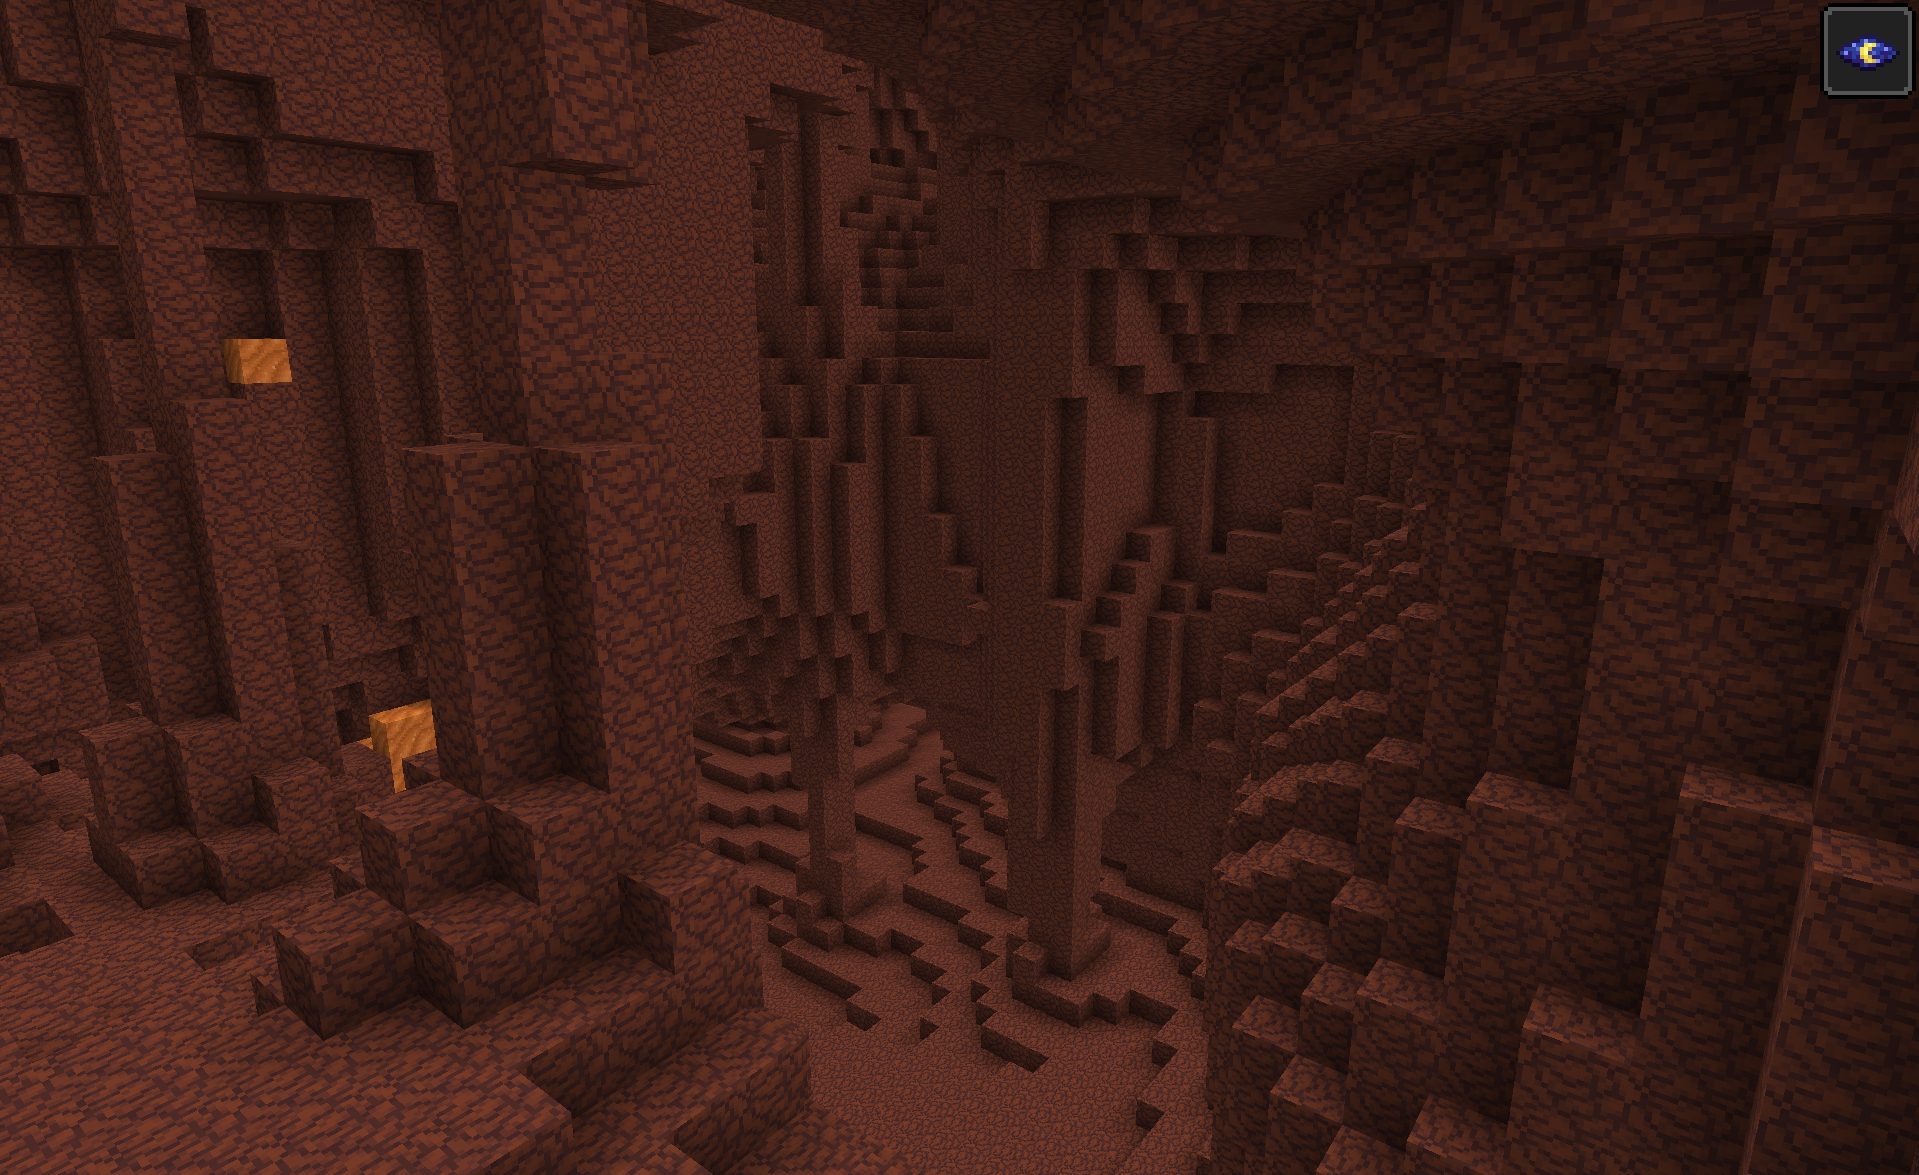
\includegraphics[width=0.75\linewidth]{images/cave.png}
    \label{fig:mars-cave}
\end{figure}

\subsubsection{Existing Structures}

Right now the only structure is a pionner outpost with a crashed ship and an minimal underground base. The loot table is relatively limited and would need improvements (right now cobalt ingot + a unique blueprint), add diversity and lore books

\subsubsection{Work remaining}

Several systems are still under development or require refinement before Mars world generation is complete.

\paragraph{Terrain and Biome Improvements}
\begin{itemize}
    \item Improve cave generation diversity and underground features.
    \item Refine mossy ravine generation and fix texture blending issues.
    \item Add surface variation to plains, including sand patches and rock formations.
    \item Improve the aquifiers, we need to have underground rivers on the side of ravines.
\end{itemize}

\paragraph{Structures and Content}
\begin{itemize}
    \item Plan and make more structures (ruins, facilities, underground complexes).
    \item Add loot tables and progression rewards tied to exploration.
\end{itemize}

\paragraph{Creatures and Flora}
\begin{itemize}
    \item Design Mars-specific mobs adapted to the desert and to the rare mossy ravines. Insect life bettles, mantas
    \item Create Martian plants for mossy and underground biomes.
    \item Define biome-based spawning rules and behaviors.
\end{itemize}

\paragraph{Future Systems}
\begin{itemize}
    \item Add dust storms and weather systems.
    \item Introduce ambient biome sounds.
    \item Expand ore and mineral generation systems.
    \item Add rare biome variants for exploration depth.
\end{itemize}

\subsection{Asteroid Belt}

The Asteroid Belt is a low-gravity environment composed of isolated asteroids suspended in space. It serves primarily as a mining and exploration region.

\subsubsection{Existing Biomes}

\begin{itemize}
    \item \textbf{Space}: A biome representing open vacuum and scattered asteroids.
\end{itemize}

\subsubsection{Existing Structures}

\begin{itemize}
    \item \textbf{Small Base}: A compact structure providing shelter and loot.
\end{itemize}

\subsubsection{Work Remaining}

\begin{itemize}
    \item Expand asteroid variety and resource distribution.
    \item Add additional structures such as mining stations and derelict spacecraft.
    \item Introduce hazards and environmental features.
    \item Add mobs
\end{itemize}


\subsection{Europa}

Europa is envisioned as an icy moon with a fractured frozen crust, subsurface oceans, and a technologically advanced native civilization.

\subsubsection{Existing Biomes}

Europa currently contains three biomes:

\begin{itemize}
    \item \textbf{Surface}: The ice crust.
    \item \textbf{Plains}: relatively flat low elevation terrain with life centered around volcanic areas / black smoker.
    \item \textbf{Volcanic Rift}: Warmer and more geologically active areas associated with tectonic fractures, bigger and more archaic life forms.
\end{itemize}

\subsubsection{Existing Structures}

No structures have been implemented yet, but future structures may include underwater cities, research stations, and structure belonging to Europa's advanced civilization.

\subsubsection{Work Remaining}

\begin{itemize}
    \item Add mobs and ecosystem-specific lifeforms.
    \item Design and implement structures.
    \item Improve aquifer behavior and subsurface ocean generation.
    \item Develop a technical solution for correctly implementing the ice crust and the ocean beneath it, take inspiration from the iceberg feature.
    \item Create custom features such as giant algae forests, hydrothermal vents, and mineral deposits.
    \item Develop the lore, architecture, and name of Europa's advanced civilization.
    \item improve the biome placement according to this image
    \begin{figure}[H]
        \centering
        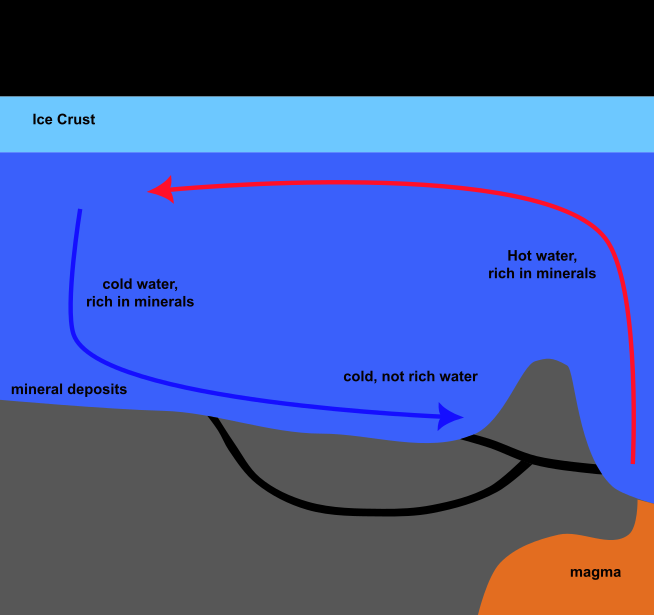
\includegraphics[width=0.5\linewidth]{images/europa_worldgen.png}
        \caption{Europa Worlden}
        \label{fig:placeholder}
    \end{figure}
\end{itemize}



\section{Textures and Visual issues}

\begin{figure}[H]
    \centering
    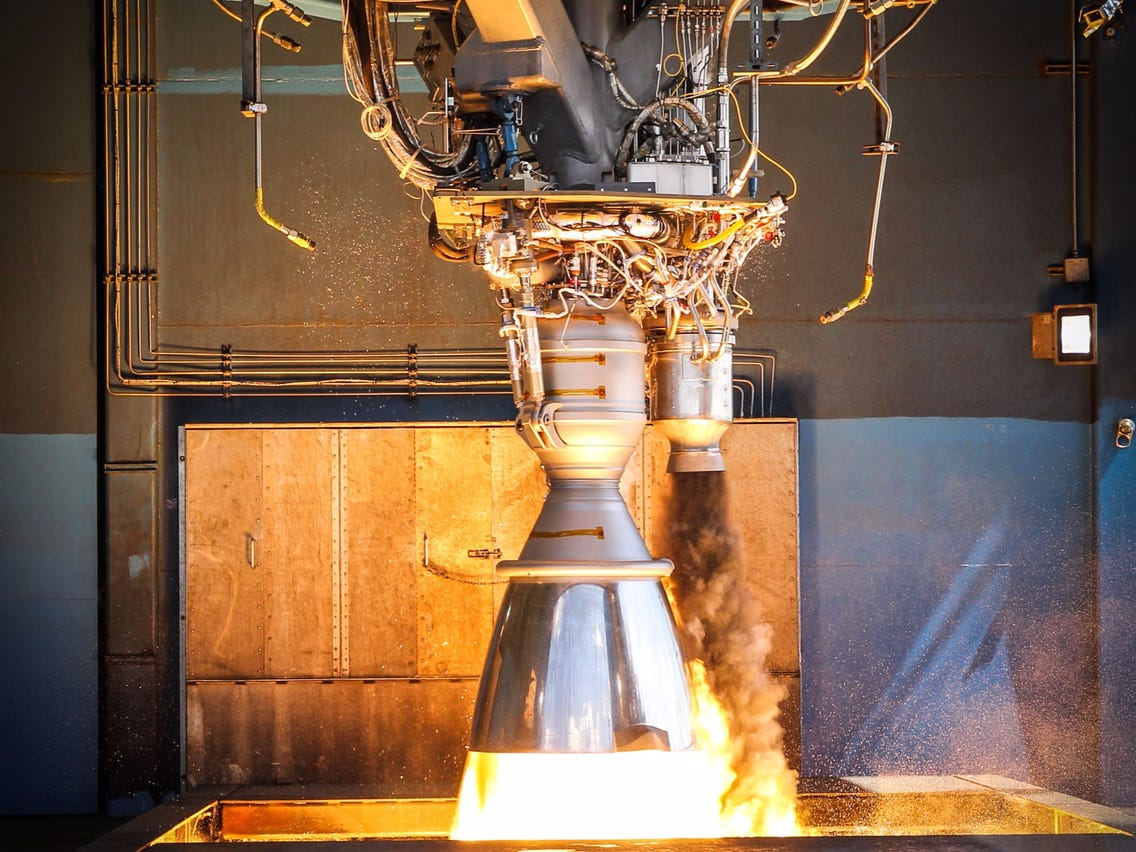
\includegraphics[width=0.75\linewidth]{images/single_turbine_engine.png}
    \caption{Single Turbine Engine}
    \label{fig:single_turbine}
\end{figure}

\begin{figure}[H]
    \centering
    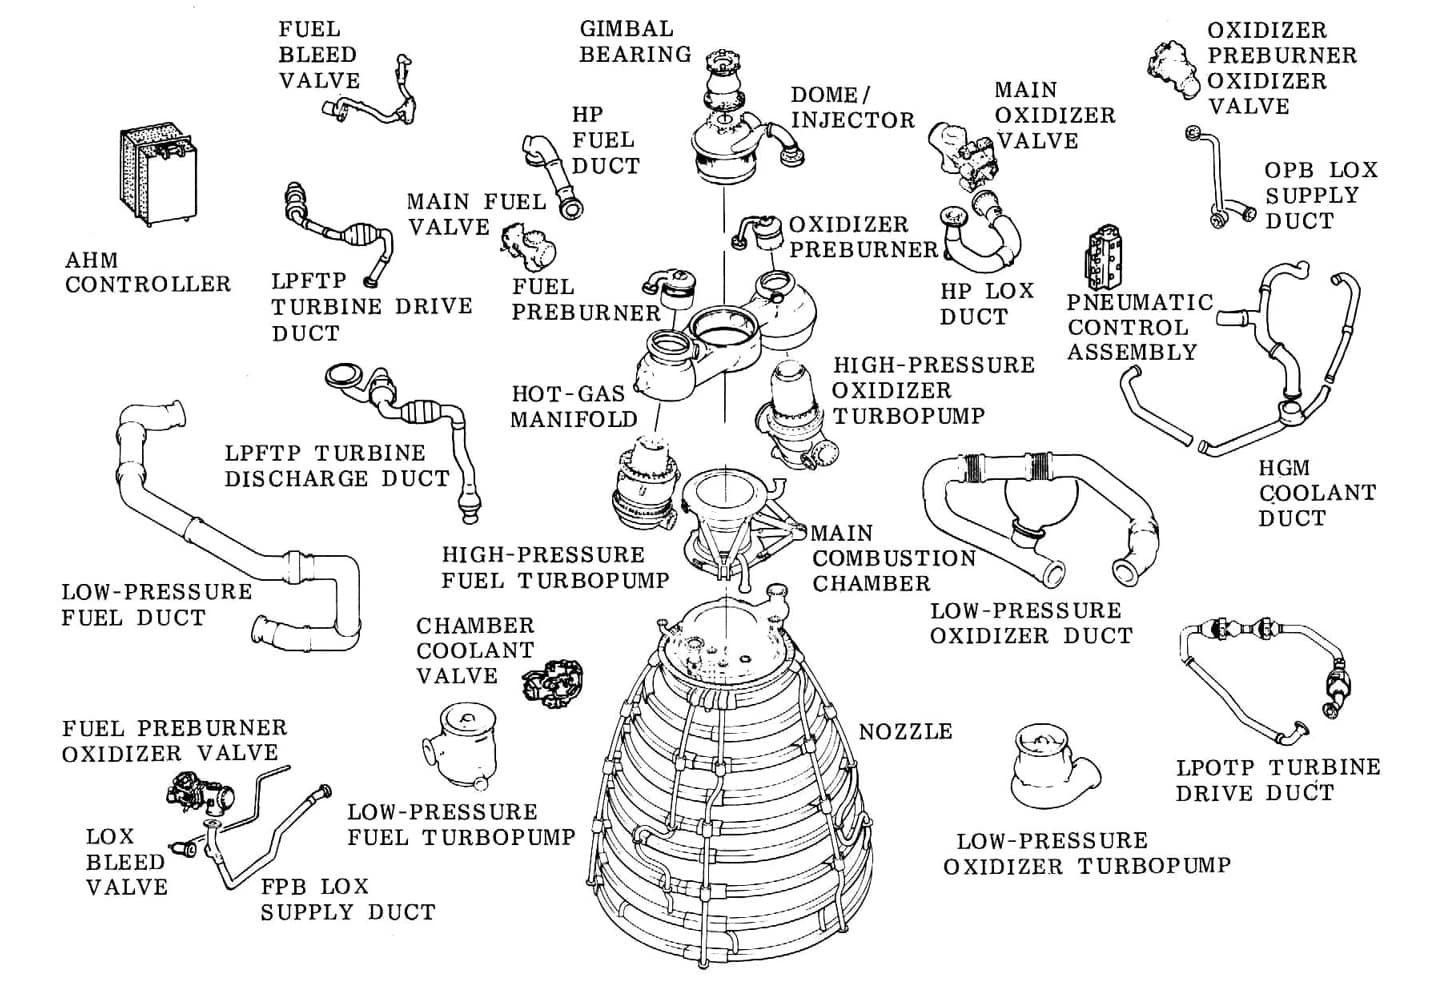
\includegraphics[width=0.75\linewidth]{images/rs25-spread_view.png}
    \caption{RS-25 spread view}
    \label{fig:rs25-1}
\end{figure}

\begin{figure}[H]
    \centering
    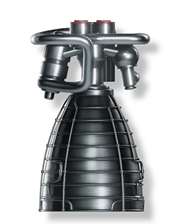
\includegraphics[width=0.25\linewidth]{images/rs25-full-view.png}
    \caption{RS-25 full view}
    \label{fig:placeholder}
\end{figure}
One issue though, is that aerospike intergrate less nicely with the rest
\begin{figure}[H]
    \centering
    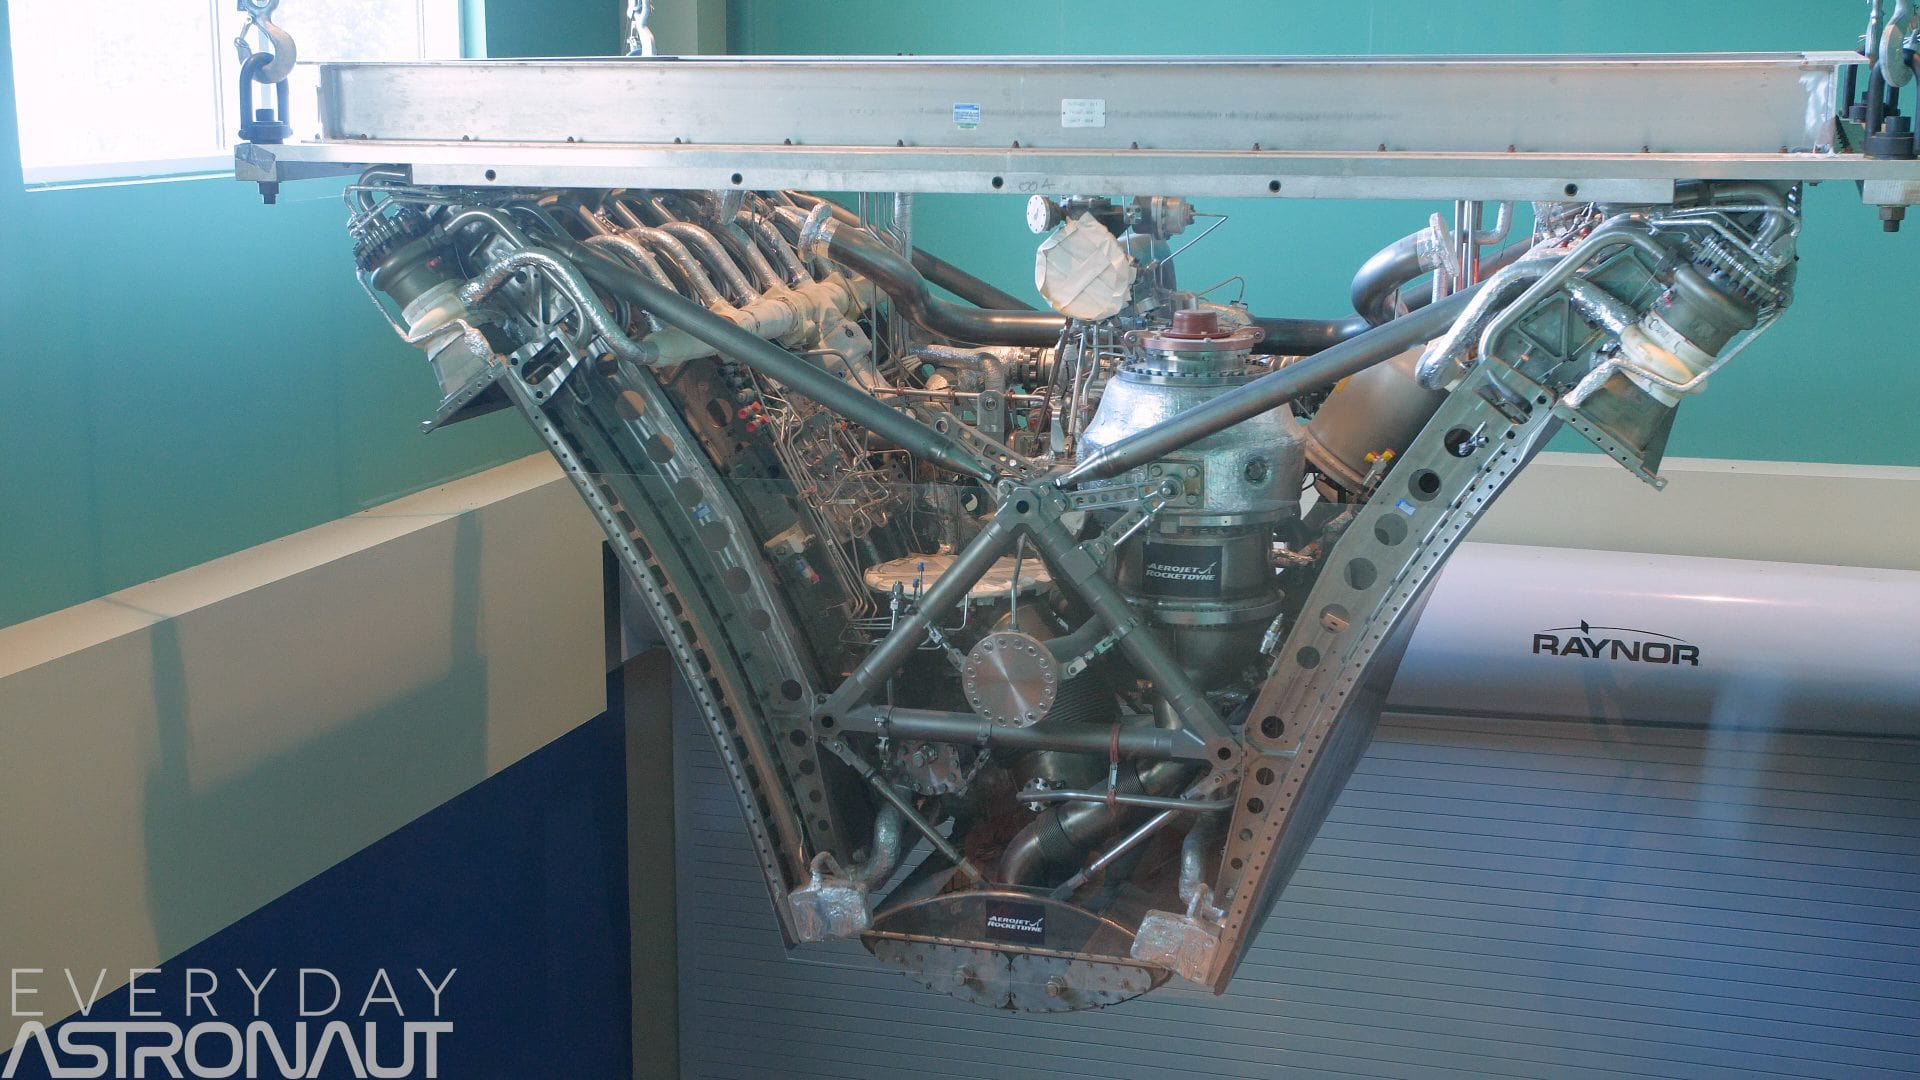
\includegraphics[width=0.75\linewidth]{images/linear_aerospike.png}
    \caption{Linear aerospike interorior}
    \label{fig:placeholder}
\end{figure}

\begin{figure}[H]
    \centering
    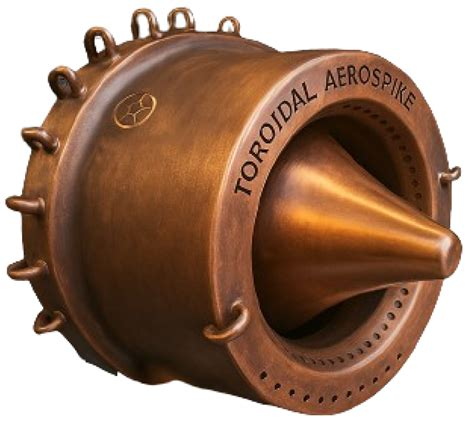
\includegraphics[width=0.50\linewidth]{images/toroidal_aerospike.png}
    \caption{Toroidal Aerospike}
    \label{fig:toroidal-aerospike}
\end{figure}

\newpage
\section{Lore}
Discution are in going bwn me and my brother on this subject.

\end{document}